\chapter{Physics Objects\label{ch:objects}}

After data is selected by the trigger, the offline analyses begin with particle identification.
There are no longer any timing limitations, so such identification can make use of all the detector
information in the event. To this end, CMS uses the Particle Flow (PF) algorithm
in most analyses, which is described in Section~\ref{sec:PF}.
As this search for double Higgs production centers around the identification of
events with both $\Hgg$ and $\Hbb$ decays, the
identification and reconstruction of photons and jets are the first steps taken after the
trigger selects potentially-interesting events,
and this chapter discusses the treatments needed at this stage for both data and MC samples.
Recalling that the sensitivity in the separation between signal and background comes from the
excellent diphoton mass resolution, the identification of two high quality photons is the starting point
and discussed in Section~\ref{sec:photons}. The following step is the identification of two jets
coming from the hadronization of b-quarks and is discussed in Section~\ref{sec:jets}.


\section{Particle Flow\label{sec:PF}}

The PF algorithm reconstructs all stable particles in an event from the digitized electronic signals
of all channels in all subsystems~\cite{PFPAS2009,CMS-PAS-PFT-10-001}. These particles include
electrons, photons, charged hadrons, neutron hadrons, and muons, as shown in Figure~\ref{fig:PF}.
From these particles, derived objects are constructed, including jets and missing transverse energy.
The algorithm itself links detector objects created from individual subsystems and groups them into
blocks that are identified with a particle. The detector objects are discussed in
Section~\ref{subsec:detobj}, the linking of these objects is discussed in Section~\ref{subsec:linking},
and the identification of groups of these links with particles is discussed in
Section~\ref{subsec:groupid}.

\begin{figure}[ht]
 \begin{center}
    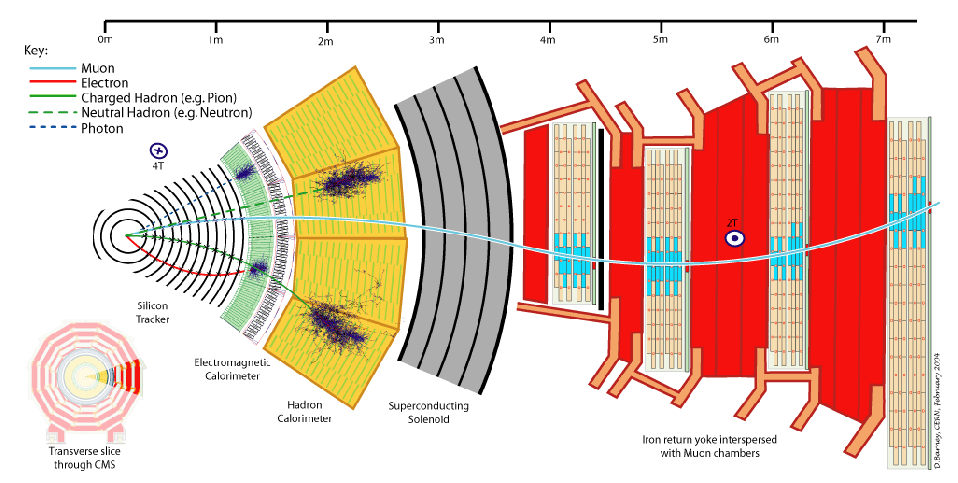
\includegraphics[width=0.95\textwidth]{figures/objects/pf.pdf}
      \end{center}
\caption{A schematic of a slice of the CMS detector in the plane transverse to the beam line.
The trajectories of an electron, photon, charged hadron, neutral hadron, and muon are superimposed
with the interactions that each of these particles has with the various subsystems.}
\label{fig:PF}
\end{figure}

\subsection{Detector Objects\label{subsec:detobj}}

The first step of the PF algorithm is to assemble detector objects created separately from
individual subsystems. In the tracker, hits in pixels or strips are associated into a track candidate
through the iterative Combinatorial Track Finder algorithm~\cite{PFPAS2009}. In the muon chambers,
standalone muon tracks (to distinguish from tracks formed by tracker hits)
are assembled from hits in the three muon detectors, accounting
for the nonuniform magnetic field and large detector budget and constraining a track candidate to
intersect the beamline. In the ECAL and HCAL, clustering of energy deposits is performed around a
cluster seed, which is identified as a detector unit with an amount of energy exceeding a
detector-dependent threshold and corresponding to a local maximum relative to neighboring units.
Units are then added to adjacent seeds if their energy exceeds a noise threshold,
and the PF clusters are
formed by redistributing the the energy back to the cluster seeds, recalculating the position as a
weighted average over the energy of each contributing cluster.

\subsection{Linking\label{subsec:linking}}

The next step of the PF algorithm is to link the detector objects to assemble PF candidates.
Possible links are between a track and standalone muon track, between a track and a cluster, and
between two clusters, each having their own associated linking parameters. A link is formed between
a track and standalone muon track when the two can be merged into a global track with a fit
having $\chi^2$ below a certain threshold. A link is formed between a track and a cluster when
the extrapolation of the track is within a certain distance of the cluster position.
A link is formed between two clusters
(either both in ECAL, both in HCAL, or one in each) when the two clusters are within a certain distance
to each other.

\subsection{Grouping and Identification\label{subsec:groupid}}

An ensemble of links creates a block, and identification proceeds iteratively through PF candidates.
First, muons are identified from those blocks that contain a global track having a momentum
sufficiently close to the momentum of the contained track. Then electrons are identified from blocks
containing a track and an ECAL cluster where the track and energy cluster satisfy requirements
consistent with the signature of an electron. Next photons and hadrons are identified from blocks
containing a track and a cluster from either ECAL or HCAL. If the calibrated energy in the clusters is
greater than the sum of the momentum of the associated tracks, PF photons or PF neutrons are created
from the difference. If the difference is less than the energy in the ECAL clusters, a PF photon is
created from the block; if the difference is greater than the energy in the ECAL clusters,
a PF photon and a PF neutral hadron are made from the excesses ECAL and HCAL energy, respectively.
Finally, if the calibrated energy in the clusters is less than the sum of the momentum of the associated
tracks, a search for fake tracks and additional muons in the block is performed, and what remains
in the block is a PF charged hadron.

From the list of PF candidates in an event, jets and taus are constructed by clustering nearby
hadrons. In this way, the clustering of PF hadrons represents the original quark or tau from the
underlying interaction. Missing transverse energy, which is a signature of one or more neutrinos
in the event and/or the mismeasurement of the energy of PF candidate, is obtained by
\begin{equation}
\met = - \sum_i \vec{p}_{{\rm T},i} \, ,
\end{equation}
where the sum is over all PF candidates in the event.

The treatment for photons is discussed in more detail in Section~\ref{sec:photons}. The construction
of jets from PF candidates is discussed in more detail in Section~\ref{sec:jets}. 


%Matching the muons to the tracks measured in the silicon tracker results in a transverse momentum
%resolution between 1 and 5\,\% for \pt values up to 1~TeV. The ECAL has an energy resolution better
%than 0.5\% for unconverted photons with transverse energies above 100~GeV.
%The HCAL, when combined with the ECAL, measures jets with a resolution
%$\Delta E/E \approx 100\,\% / \sqrt{E\,[\gev]} \oplus 5\,\%$.

\section{Photons\label{sec:photons}}

PF photon candidates are reconstructed from clustering individual units in the ECAL
and checking consistency with tracks.
The calorimeter signals are calibrated for several detector effects~\cite{CMS-PAS-EGM-10-005,ECALpaper},
providing the best energy resolution possible.
The energy scale is corrected in both data and simulation, while the photon energy is smeared in
simulation in order to reproduce the same energy resolution that is observed in data.

With the PF photon candidates in hand, additional requirements are imposed in order to further
separate prompt photons from fake photons originating from misidentified electrons or from jets.
These additional requirements include an electron veto, an upper threshold on the energy deposited
in HCAL in the region about the candidate, isolation, and the shower shape. The electron veto 
removes a photon if there is an electron candidate matching the photon ECAL cluster with no missing
hits in the tracker and with no matching reconstructed conversion.
Isolation requirements place
thresholds on the amount of ECAL energy deposited in a region about the cluster; these are both
detector based and PF based. Requirements on the electromagnetic shower shape include the
width of the shower in terms of ECAL detector units and
ratio of the amount of energy in a 3$\times$3 unit box around the cluster seed to that
around a 5$\times$5 unit box.

After the quality cuts, the two photons candidates are requested to satisfy the sliding asymmetric cuts
\begin{subequations}
\begin{equation}
p_{{\rm T},\gamma_1} > \frac{\Mgg}{3}
\end{equation}
\begin{equation}
p_{{\rm T},\gamma_2} > \frac{\Mgg}{4} \, ,
\end{equation}
\end{subequations}
where $p_{{\rm T},\gamma_1}$ and $p_{{\rm T},\gamma_2}$ are the transverse momenta of the
leading and subleading photons, respectively.
The fact that these requirements on the transverse momentum are scaled by the diphoton invariant mass
prevents turn-on effects which could distort the shape of the $\Mgg$ spectrum for low values of $\Mgg$.
Both photons have the requirement that their position be within the ECAL acceptance of
$\left|\eta\right| < 2.5$ with an exclusion on the ECAL gap between the barrel and endcaps.
In the case that there are more than two photons passing the identification and kinematic requirements,
the two with the largest $p_{\rm T}$ are chosen. After this choice, the diphoton mass is required to
be between 100 and 180 GeV.

Figure~\ref{fig:mgg_onlyhiggs} shows the resulting simulated distributions for the diphoton mass 
of the resonant signal and resonant backgrounds.
In the case of the resonant background, the sum
of all SM $\Hgg$ production mechanisms is shown as a single contribution.
Figure~\ref{fig:mgg_controlplot} shows the same
distribution for data and the sum of backgrounds. (Note that these figures include requirements
on jets, discussed in Section~\ref{sec:jets}.)
The resolution of the diphoton mass spectrum for the signal is a few GeV.

The two primary drivers in the diphoton mass resolution are the energy resolution
of the individual photons
and the direction of the photons from their origin, which is synonymous with the identification
of the vertex from which they were produced. Due to the presence of the $\Hbb$ decay in the search,
the tracks from the jets allow for the efficient identification of the correct vertex since photons
do not have tracks unless they undergo pair-conversion in the tracker.
The criterion for the vertex choice is that which has the largest $\sum_i p_{{\rm T},i}$, where
the sum is over all of the tracks associated to a particular vertex. With this criterion,
the relative contribution to the diphoton mass resolution due to the vertex choice is
negligible with respect to the energy resolution for individual photons.

\begin{figure}[ht]
 \begin{center}
   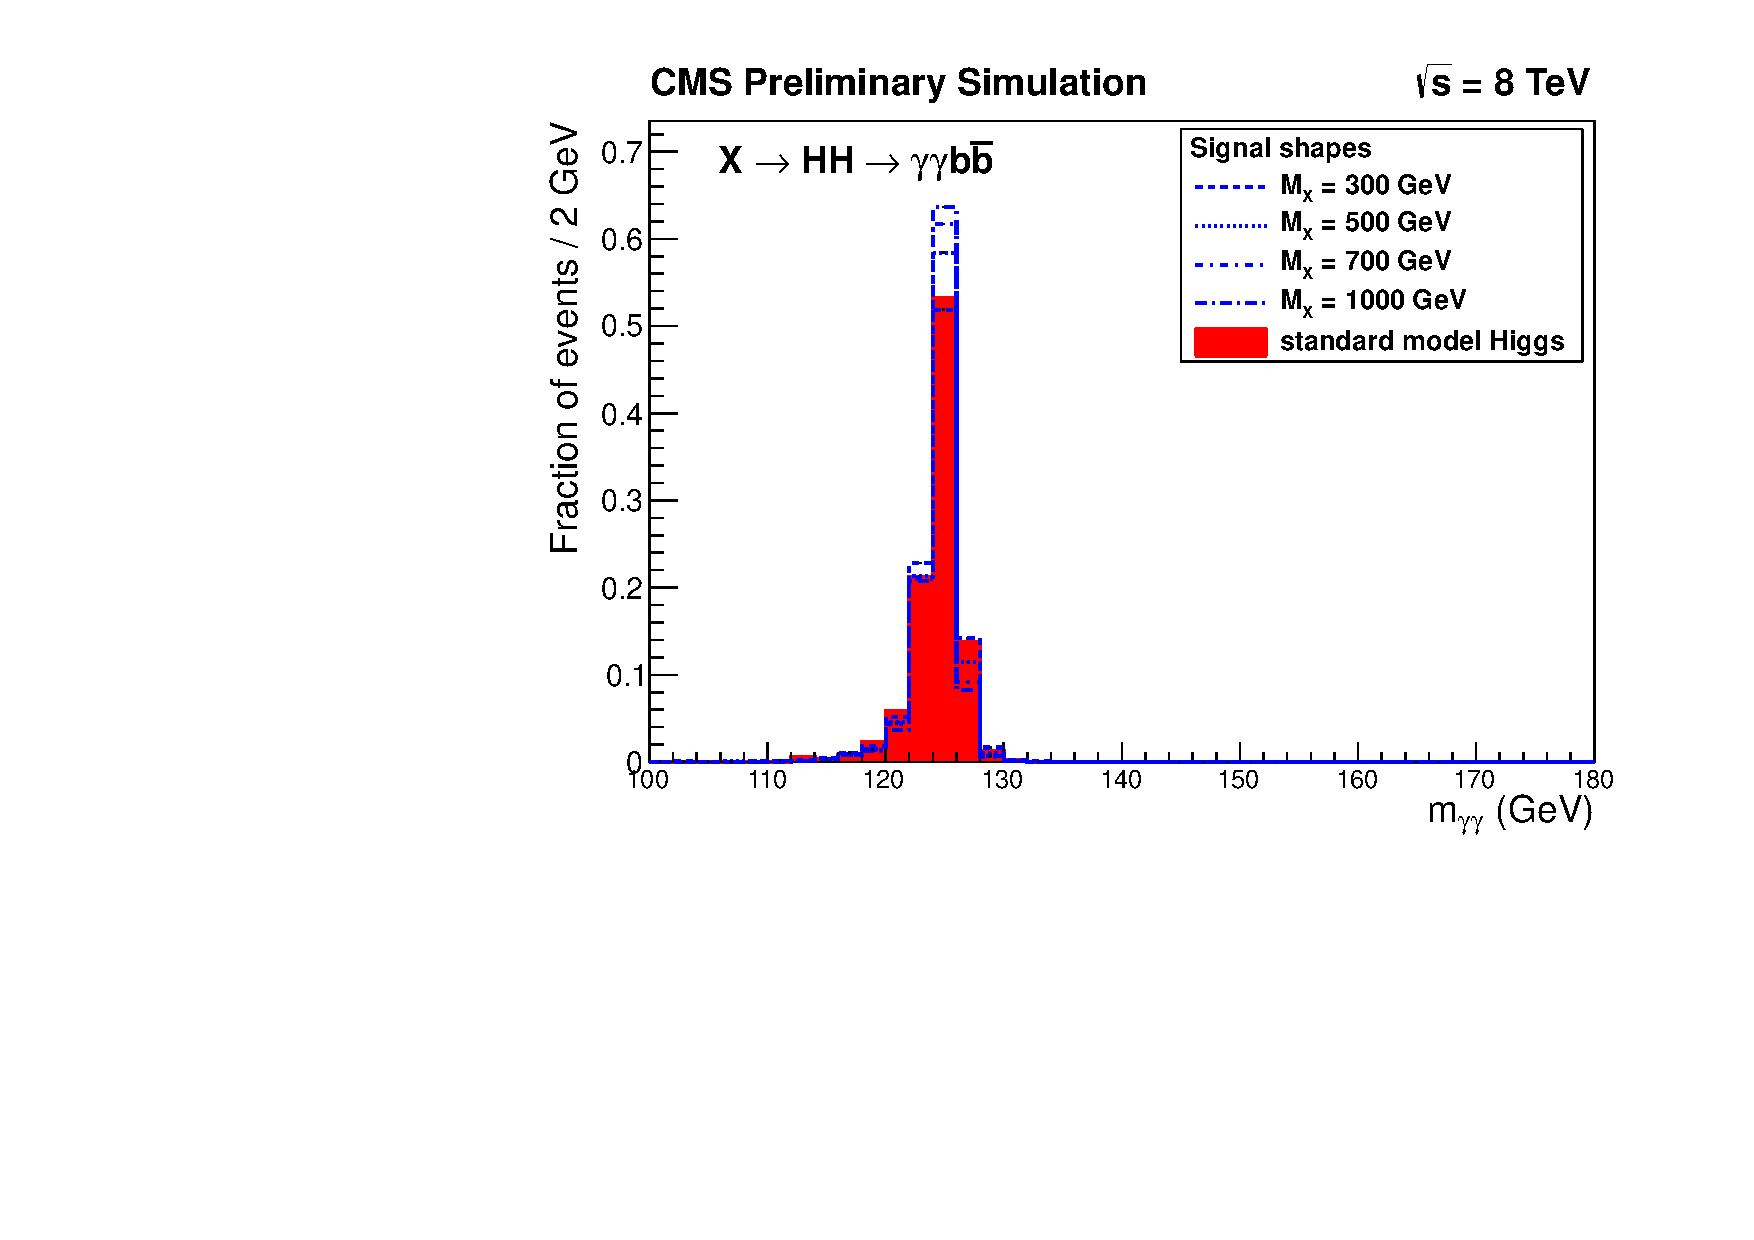
\includegraphics[width=0.70\textwidth]{figures/objects/DiPhotonMass_OnlyHiggs.pdf}
 \end{center}
\caption{Simulated diphoton mass spectrum for the resonant signal and the sum of all production
mechanisms of the
SM Higgs boson after basic selections on photons and jets and requesting at least
one loose b-tagged jet.
The spectra are normalized to one.}
\label{fig:mgg_onlyhiggs}
\end{figure}

\begin{figure}[ht]
 \begin{center}
   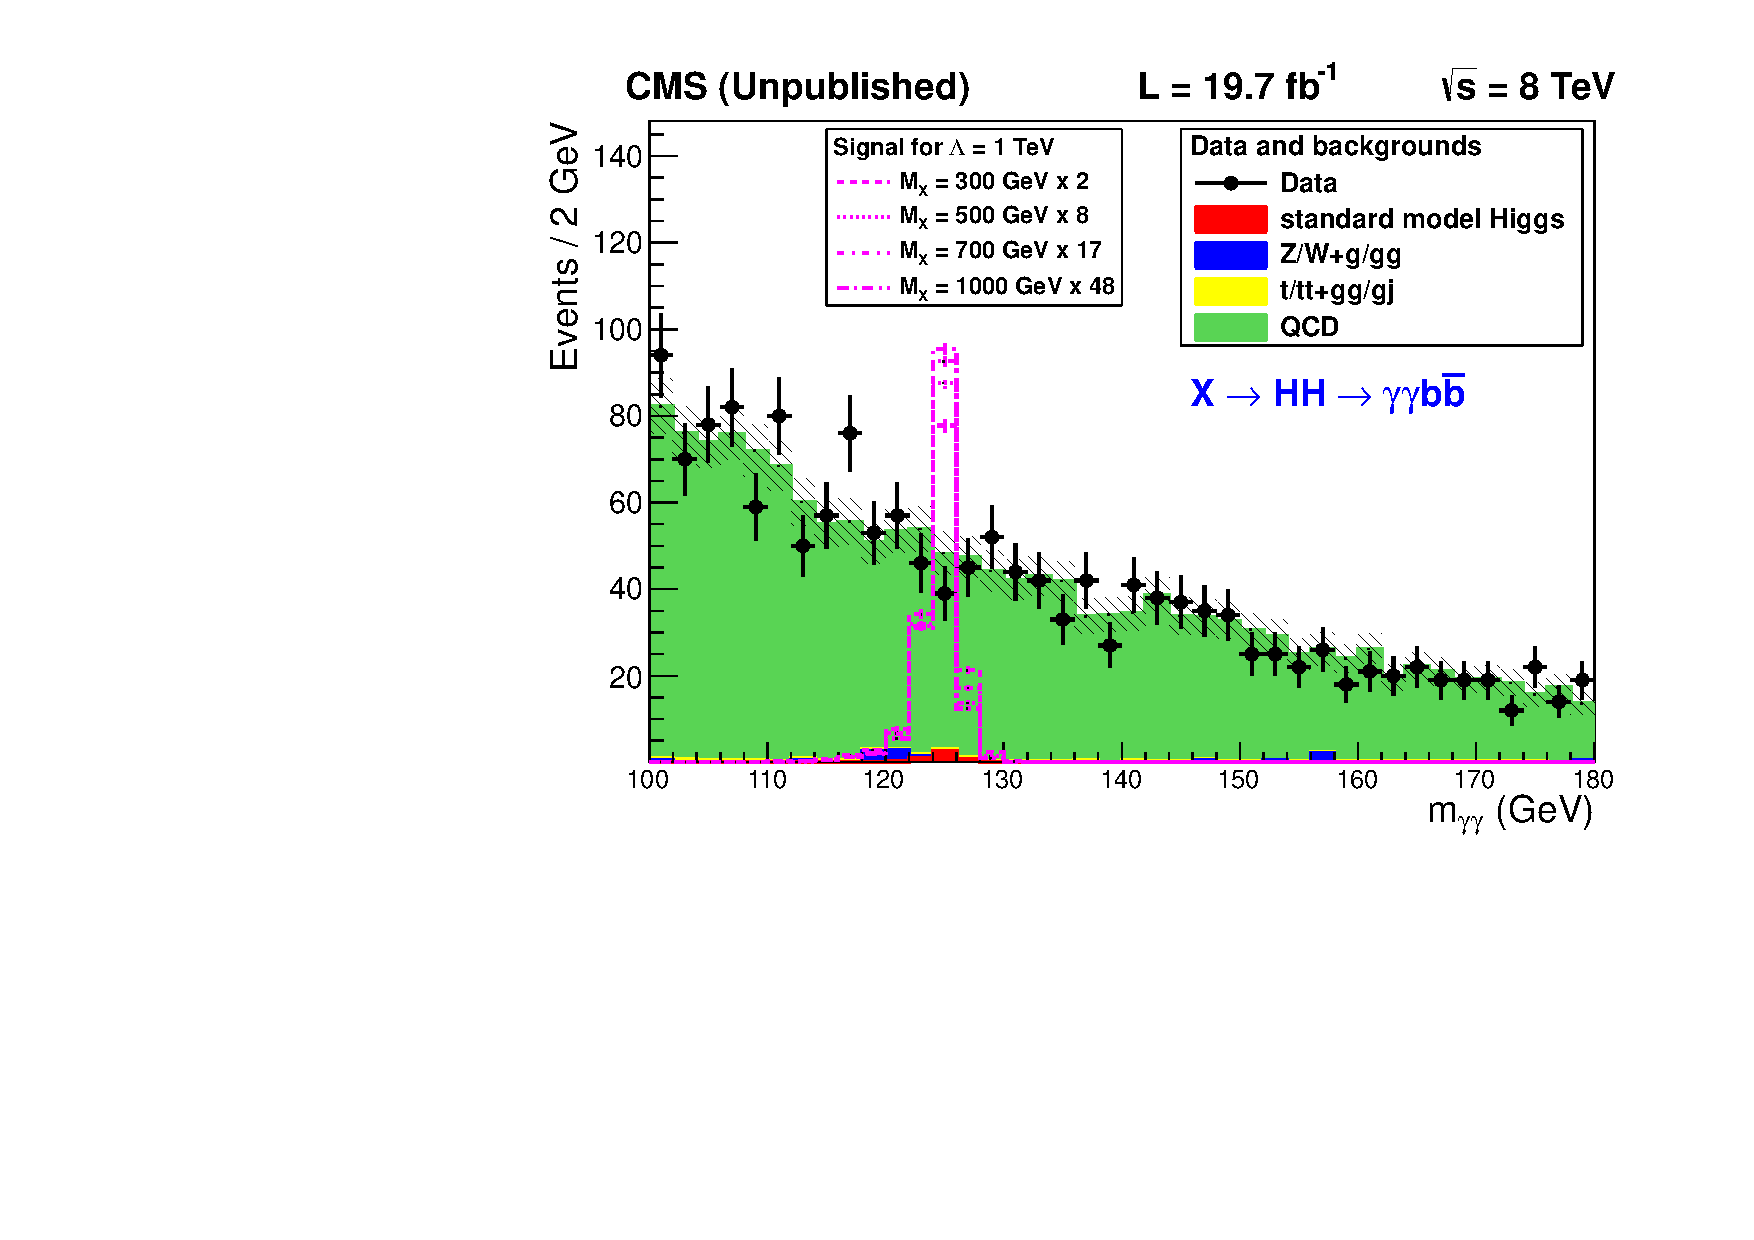
\includegraphics[width=0.70\textwidth]{figures/objects/DiPhotonMass_ShapeNormalized_sys.pdf}
   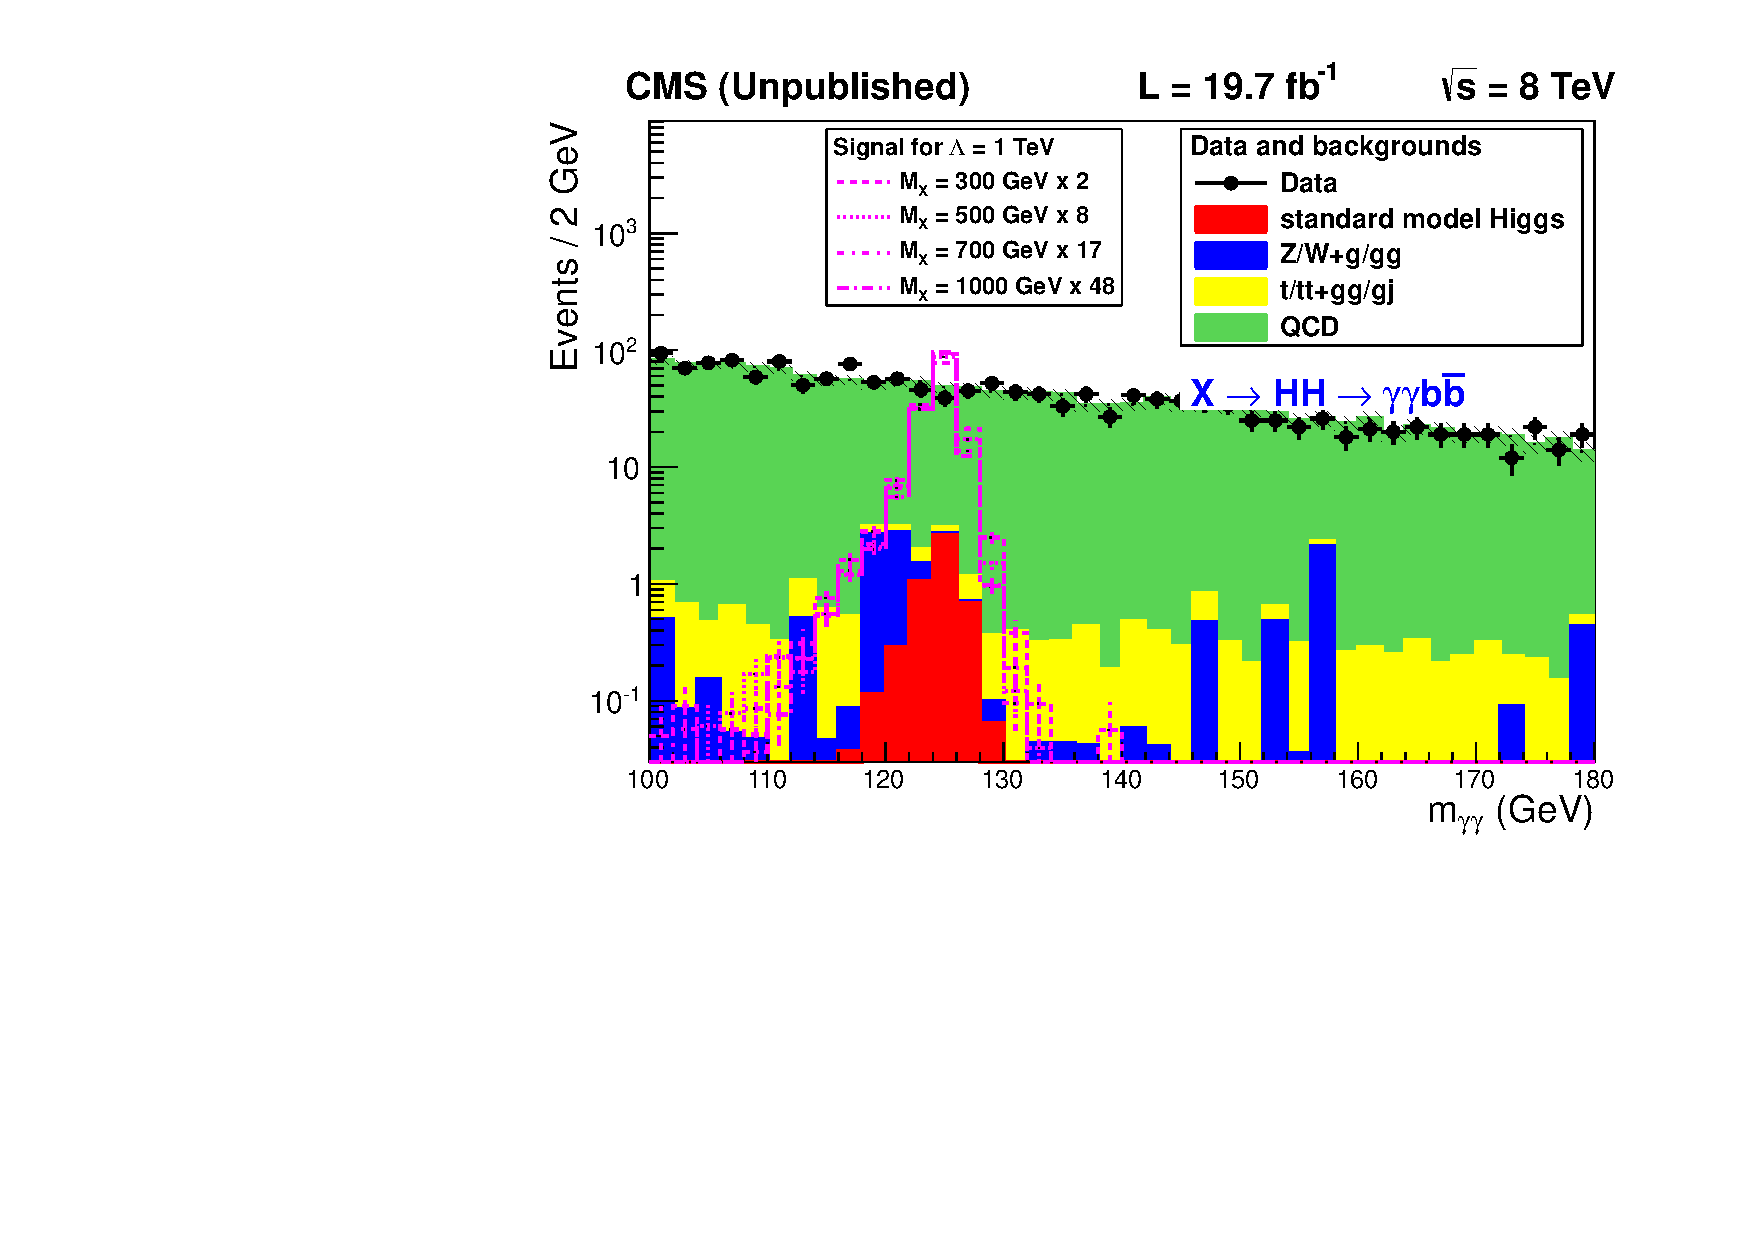
\includegraphics[width=0.70\textwidth]{figures/objects/DiPhotonMass_ShapeNormalized_Log_sys.pdf}
 \end{center}
\caption{Control plots for the diphoton mass spectrum after basic photon and jet selections
and requiring at least one loose b-tagged jet. The simulation is normalized to data and
the statistical uncertainty on the number of simulated events is shown in dashed overlay.
The top (bottom) figure is shown in linear (log) scale.}
\label{fig:mgg_controlplot}
\end{figure}

\section{Jets\label{sec:jets}}

PF jet reconstruction involves the clustering of all PF candidates except the two photons selected
as the $\Hgg$ candidate~\cite{PFPAS2009,CMS-PAS-PFT-10-001}.
The anti-$k_{\rm T}$ algorithm~\cite{Cacciari:2008gp} with a distance parameter of $R = 0.5$ is
used to cluster the PF candidates into jets as an approximate attempt to reverse engineer the
processes of hadronization and fragmentation after a b-quark was produced in the interaction.
In this greedy algorithm, a list of particles and pseudojets is maintained, and at each iteration
elements $i$ and $j$ are combined into one pseudojet if that pair has the minimum distance measure
in the list, where the distance measure $d_{ij}$ is defined as
\begin{equation}
d_{i,j} = \min \left(\frac{1}{k_{{\rm T},i}^2},\frac{1}{k_{{\rm T},j}^2}\right)\frac{\Delta R_{i,j}^2}{R^2} \, ,
\end{equation}
where $k_{{\rm T},i}$ is the transverse momentum of $i$ and $\Delta R_{i,j} = \sqrt{(\eta_i-\eta_j)^2+(\phi_i-\phi_j)^2}$ is the angular separation between $i$ and $j$. If, on a particular iteration,
$d_{i,B}$ is the minimum, defined as
\begin{equation}
d_{i,B} = \frac{1}{k_{{\rm T},i}^2} \, ,
\end{equation}
then element $i$ is considered a jet and is removed from the list. The algorithm continues until the
list is empty.
The advantages of this clustering algorithm is that harder jets tend to be reconstructed as circles
in the $\eta\times\phi$ plane and that the clustering is not sensitive to
hadronization from pileup and the underlying event.

After the jet reconstruction, the energy is corrected for pileup contributions from both the same
bunch crossing and neighboring bunch crossings. This is accomplished with the the
jet area technique~\cite{Cacciari:2007fd} carried out by the FastJet package~\cite{Cacciari:2011ma}
in which the jet $p_{\rm T}$ is corrected per unit area based on an event-by-event estimation of pileup
activity.
Jet energy is further corrected as a function of the jet $p_{\rm T}$ and $\eta$~\cite{JINST6}
due to potential mismeasurement and the presence of neutrinos.

Additional requirements are imposed to reject jets that originate from detector noise or from the
clustering of particles due to pileup in favor of those that originate from a parton in the
primary interaction~\cite{CMS-PAS-JME-13-005}. Two criteria used are based on the fraction
of charged PF candidates attached to the primary vertex $\beta^*$ and the jet width
$\langle\Delta R^2\rangle$, defined as
\begin{subequations}
\begin{equation}
\beta^* = \frac{\sum_{i\in \text{other PV}} p_{{\rm T},i}}{\sum_{i\in\text{charged}} p_{{\rm T},i}}
\end{equation}
\begin{equation}
\langle\Delta R^2\rangle = \frac{\sum_i \Delta R_i^2 p_{{\rm T},i}^2}{\sum_i p_{{\rm T},i}^2} \, ,
\end{equation}
\end{subequations}
where ``other PV'' refers to the PF charged candidates associated to another primary vertex, the sum
in the denominator of $\beta^*$ is over the charged candidates in the jet, the sums
in $\langle\Delta R^2\rangle$ are over all constituents in the jet, and $\Delta R_i$ is the
angular distance between constituent $i$ and the jet axis. Upper thresholds are imposed on these
quantities; in the case of $\beta^*$ the threshold is a function of the number of reconstructed
vertices.

The efficiency of the jet identification from the above criteria exceeds 95\%. Additional kinematic
requirements on the jets include $p_{\rm T} > 25$~GeV and $|\eta| < 2.5$ (within the tracker
acceptance). In the case that more than two jets pass identification and kinematic selections, the
two jets with the highest $p_{{\rm T},jj}$ are chosen to make the dijet candidate, which will
be discussed in more detail in Section~\ref{sec:higgsreconstruction}.
Figure~\ref{fig:mjj_onlyhiggs} shows the resulting simulated distributions for the
dijet mass of the resonant signal and resonant backgrounds.
Figure~\ref{fig:mjj_controlplot} shows the same
distribution for data and the sum of backgrounds. (Note that these figures include a requirement
on the compatibility of one of the jets coming from a b-quark, discussed in Section~\ref{subsec:btag}.)


\begin{figure}[ht]
 \begin{center}
    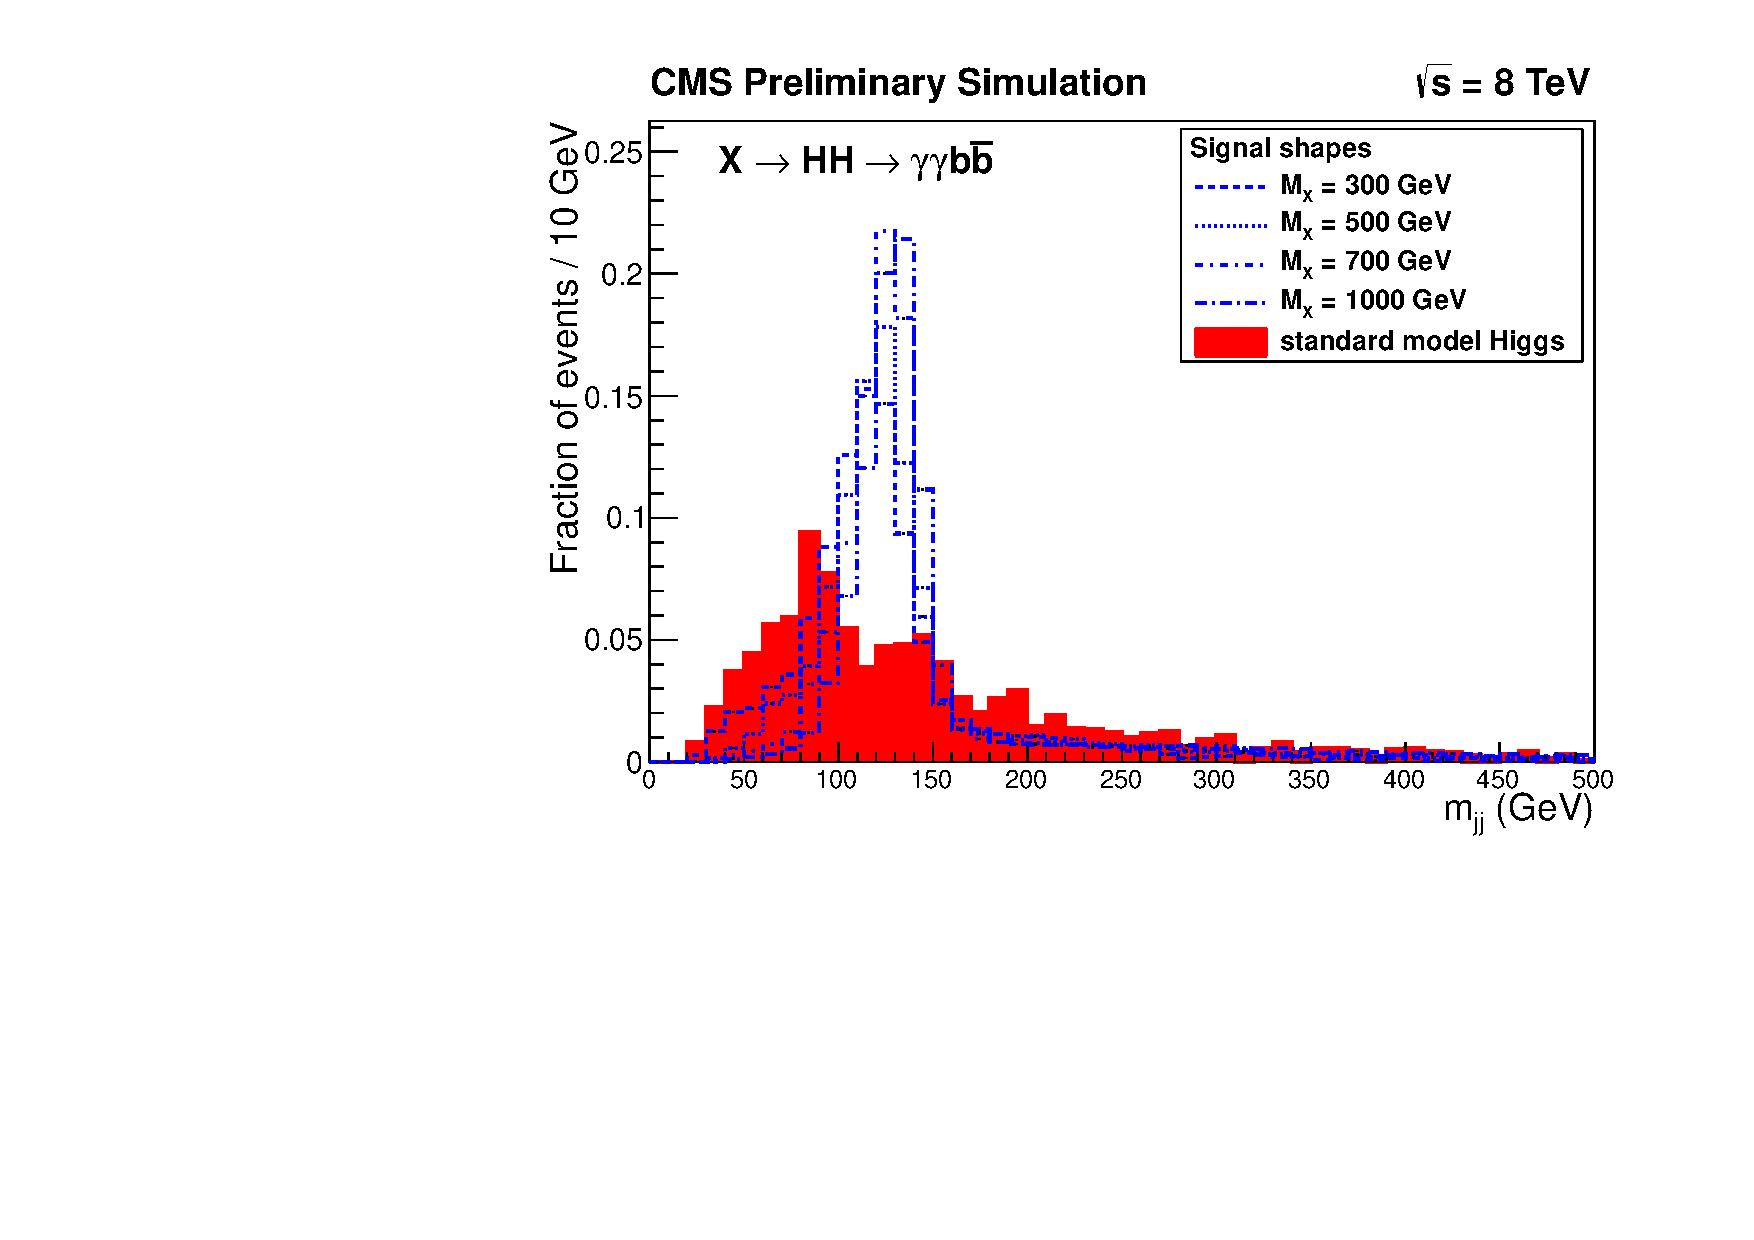
\includegraphics[width=0.70\textwidth]{figures/objects/DiJetMass_OnlyHiggs.pdf}
 \end{center}
\caption{Simulated dijet mass spectrum for the resonant signal and the sum of all production
mechanisms of the
SM Higgs boson after basic selections on photons and jets and requesting at least one loose
b-tagged jet.
The spectra are normalized to one.}
\label{fig:mjj_onlyhiggs}
\end{figure}

\begin{figure}[ht]
 \begin{center}
   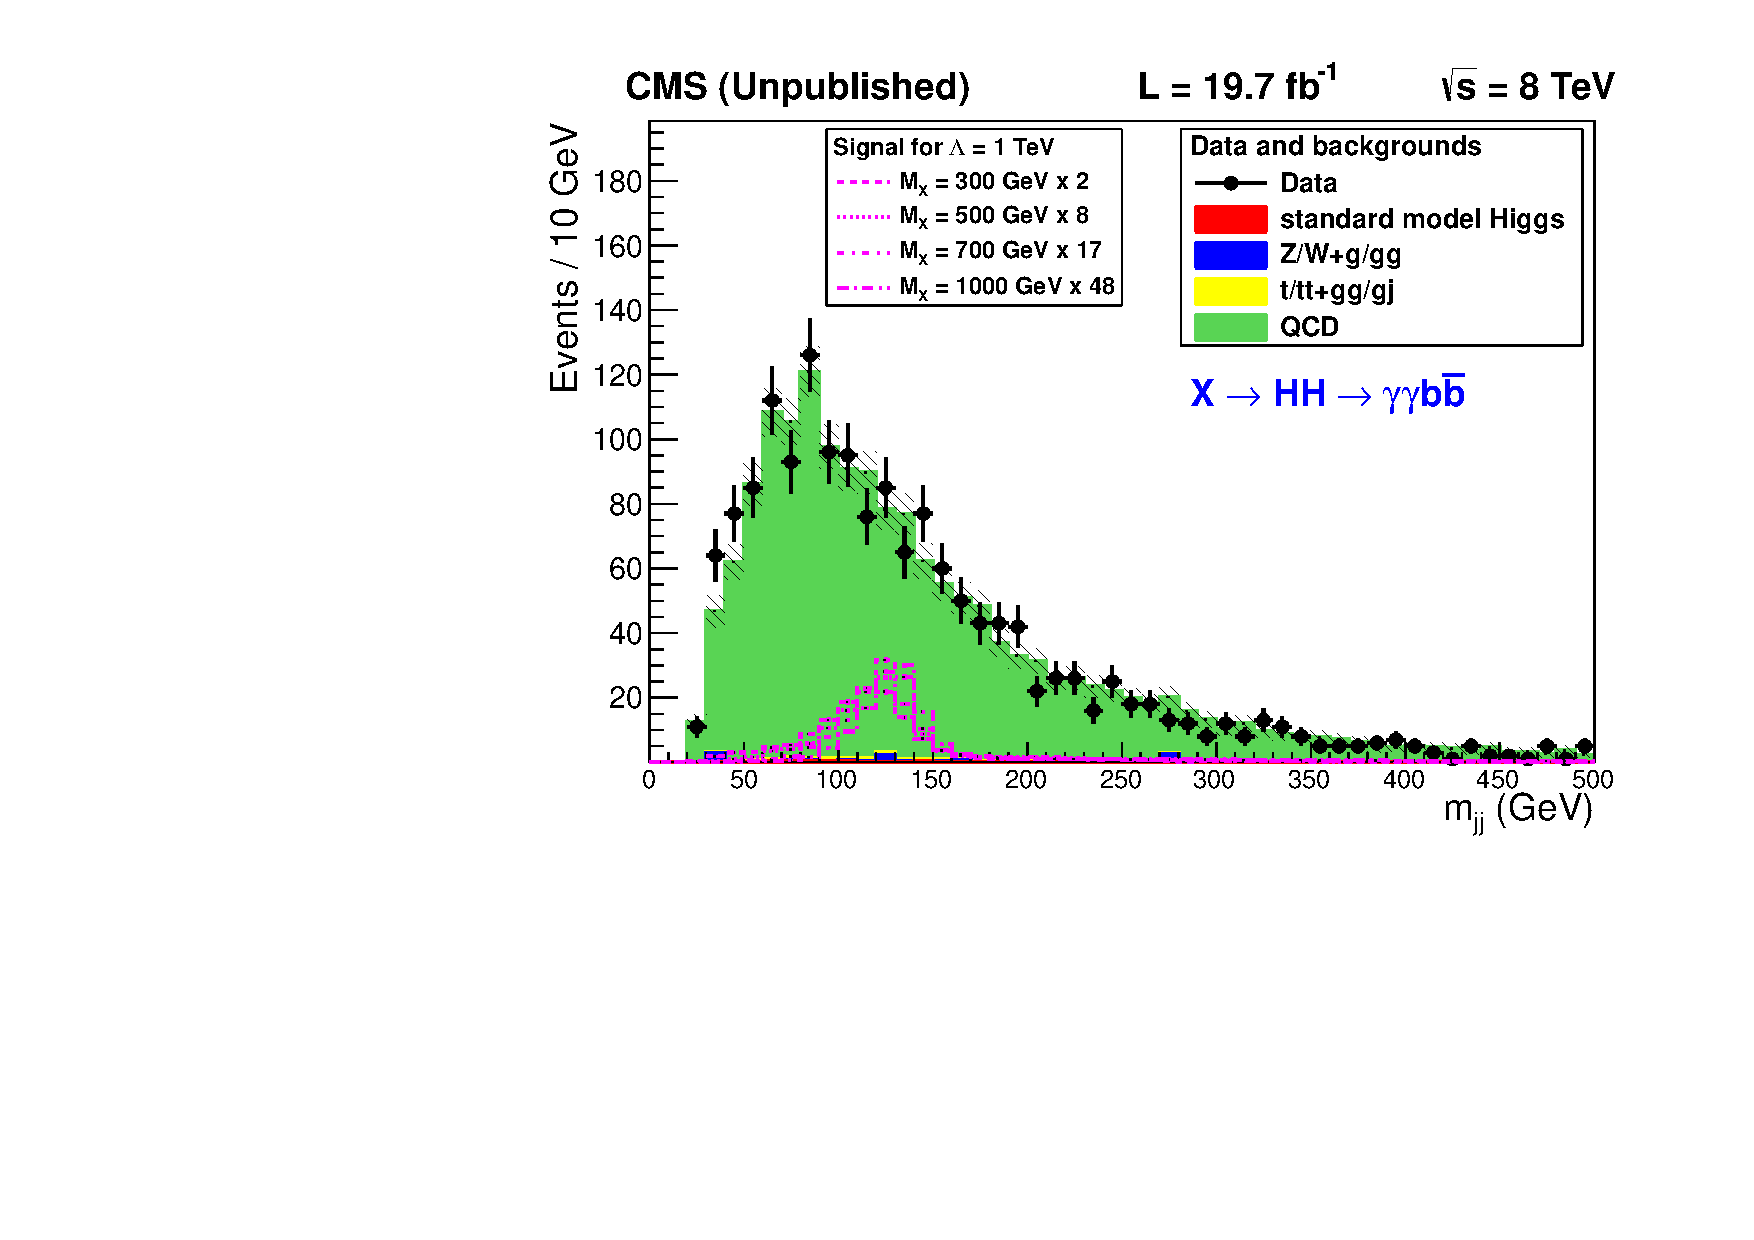
\includegraphics[width=0.70\textwidth]{figures/objects/DiJetMass_ShapeNormalized_sys.pdf}
   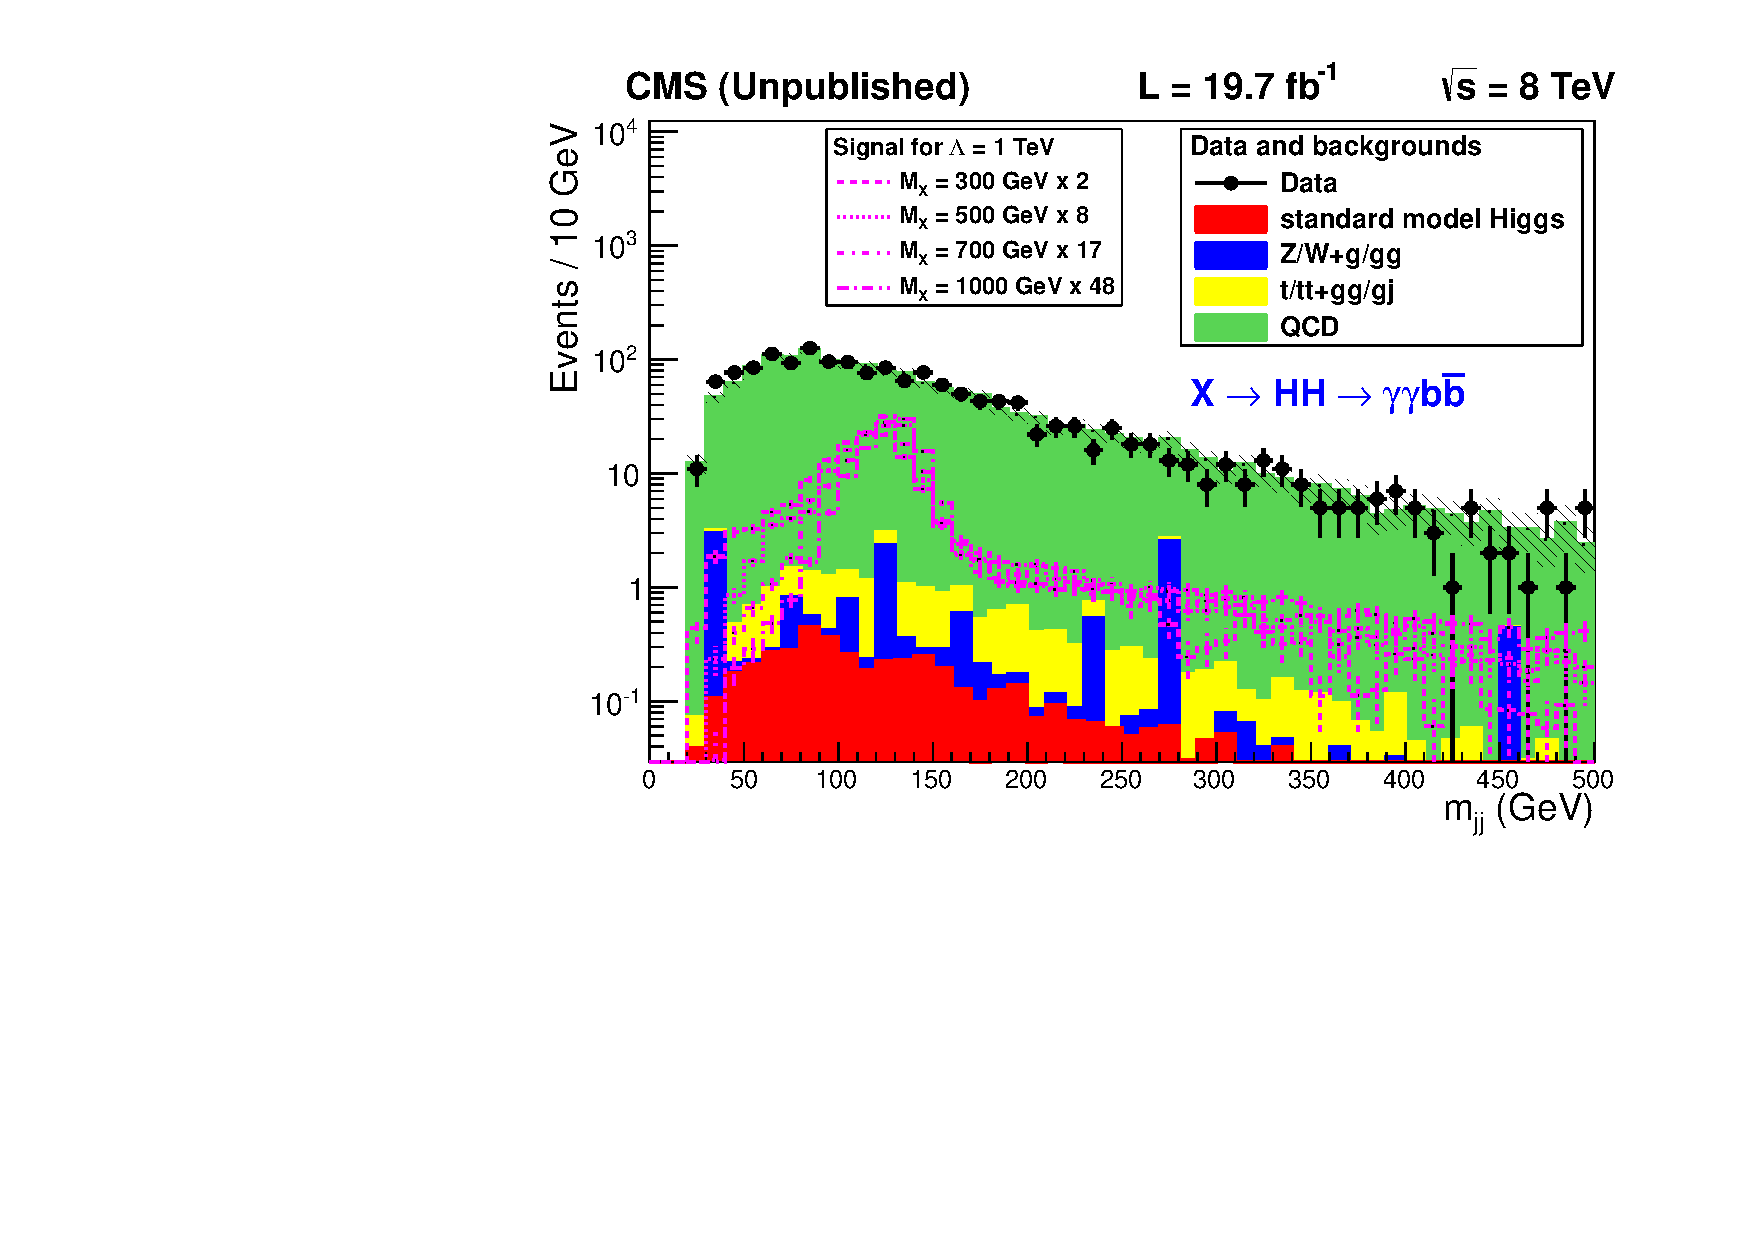
\includegraphics[width=0.70\textwidth]{figures/objects/DiJetMass_ShapeNormalized_Log_sys.pdf}
 \end{center}
\caption{Control plots for the dijet mass spectrum after basic photon and jet selections
and requiring at least one loose b-tagged jet. The simulation is normalized to data and
the statistical uncertainty on the number of simulated events is shown in dashed overlay.
The top (bottom) figure is shown in linear (log) scale.}
\label{fig:mjj_controlplot}
\end{figure}

\subsection{B-tagging\label{subsec:btag}}

The relatively long lifetime of B mesons, coming from the production of a b-quark in the event,
means that these mesons travel around $500~\mu m$ on average before decaying into more stable
light-flavor hadrons.
This property is exploited by looking for tracks consistent with a secondary vertex from
the B-meson decay and allows for further discrimination between signal and background events.
The Combined Secondary Vertex (CSV) b-tagger~\cite{BTV} combines
information from track impact parameters and secondary vertices within a given jet, and
provides a continuous output which provides discrimination between jets coming from the
hadronization of a b-quark against light-flavor and gluon jets.
The efficiency to tag b-jets and the rate of misidentification depends on the chosen threshold
of the CSV output and are measured in data samples enriched in b-jets, for example in $t\bar{t}$ events.
The simulation samples are corrected by applying event weights to account for the
differences between data and simulation with respect to the b-tag efficiency.
At preselection level, one loose b-tagged jet (CSVL) is required in the event, which corresponds to
a mistag rate of 10\%.

\subsection{Jet Energy Regression}

The jet energy corrections are performed globally on average for all jets, whereas the jets in
the signal of interest originate from the hadronization of b-quarks. Therefore, the correction
can be improved by exploiting the properties of these jets, which will in turn improve the resolution
of the dijet mass. A motivation for implementing an additional correction is to improve separation
between signal and background, particularly against
the resonance background $Z(b\bar{b})H(\gamma\gamma)$,
since the mass of the Z is very close to that of the Higgs relative to the dijet mass resolution.

Here a jet energy regression is presented, which acts as a multidimensional calibration tuned to the
specific jet properties of the signal. It is not used in the final analysis, but it can serve
as a 10--20\% improvement in sensitivity of the low-mass resonant signal
for future iterations of the analysis.

The correction comes from training a Boosted Decision Tree (BDT) regression simultaneously
on half of the MSSM signal
samples at resonant masses of 260, 300, and 350 GeV; these samples were previously
discussed in Section~\ref{subsec:sig_samples}.
These samples are generated with about 50k events each and are independent of the Radion
samples on which the final limits are extracted.

The regression is trained on every jet passing the identification criterion and the
following kinematic criteria:
\begin{itemize}
\item $p_T > 20$~GeV,
\item $|\eta|<2.5$, and
\item $\Delta R (j, j_\text{gen}) < 0.4$ (the angular separation between the jet and its associated
generator-level jet).
\end{itemize}                                                                                           
The $p_T$ threshold is increased to 25 GeV for testing and implementation.

The BDT algorithm is implemented from the TMVA package~\cite{TMVA2007} using gradient boost.
The input variables are
\begin{itemize}
\item the jet transverse momentum $p_T$,
\item the jet transverse mass $m_T$,
\item the jet pseudorapidity $\eta$,
\item the jet PF photon energy fraction,
\item the jet PF neutral hadron energy fraction,
\item the number of PF jet constituents (both charged and neutral),
\item the lead track $p_T$ associated to the jet,
\item the jet secondary vertex flight distance error (if there is a secondary vertex),
\item the jet secondary vertex mass (if there is a secondary vertex),
\item the soft lepton $p_T$ (if there is a soft lepton in the jet),
\item the soft lepton relative $p_T$ in direction of the jet (if there is a soft lepton in the jet),
\item PF $\met$ with $\Hgg$ specific corrections~\cite{HggCMS},
\item $\Delta \phi (j, \met)$, and
\item the median jet energy per jet area $\rho$. 
\end{itemize}
The secondary vertex refers to that of the B-meson decay, if such a vertex was identified.
The soft lepton refers to an electron or muon resonstructed inside the cone of the jet.

The figure of merit to quantify the effect of the regression is the resolution improvements
measured in the dijet and four-body ($\ggjj$) mass spectra of the signal sample.
Possible overtraining has been studied and considered negligible.
The resolution improvements in the \Mjj\, and \Mggjj\, spectra are quoted through a
fit to each spectrum using the sum of a Crystal Ball and third-order polynomial for events
in both 1-tag and 2-tag categories, which will be discussed in Section~\ref{sec:classification}.
The parameters of the Crystal Ball give estimates
of the spread and central value of the distribution, and the ratio of these two gives the resolution.
Table~\ref{table:regression_improvement_res} shows in improvement in the resolution separately
for the two spectra and for the two event categories.
The improvement is shown visually in the $\Mjj$ spectrum in
Figure~\ref{fig:regression_plots_improvement_mjj} where both event categories are combined.

\begin{table}[ht]
  \centering
  \renewcommand{\arraystretch}{1.4}
  \caption{Improvement from the regression on $\Mggjj$ and $\Mjj$ spectra, divided into 1-tag or 2-tag
categories. (Categorization is discussed in Section~\ref{sec:classification}.)
All numbers are in units of percentage.}
  \begin{tabular}{c||c|c|c|c|}
 & \multicolumn{2}{|c|}{\Mggjj\, spectrum} & \multicolumn{2}{|c|}{\Mjj\, spectrum} \\\hline
$m_X$ (GeV) & 1-tag & 2-tag & 1-tag & 2-tag \\ \hline
270 & 19.72 & 3.10  & 15.08 & 12.24 \\  
300 & 16.64 & 8.70  & 16.05 & 14.19 \\  
350 & 19.76 & 13.62 & 23.07 & 18.95 \\  
400 & 19.82 & 21.23 & 17.03 & 14.74 \\ 
\end{tabular}

  \label{table:regression_improvement_res}
\end{table}

\begin{figure}[ht]
\begin{center}
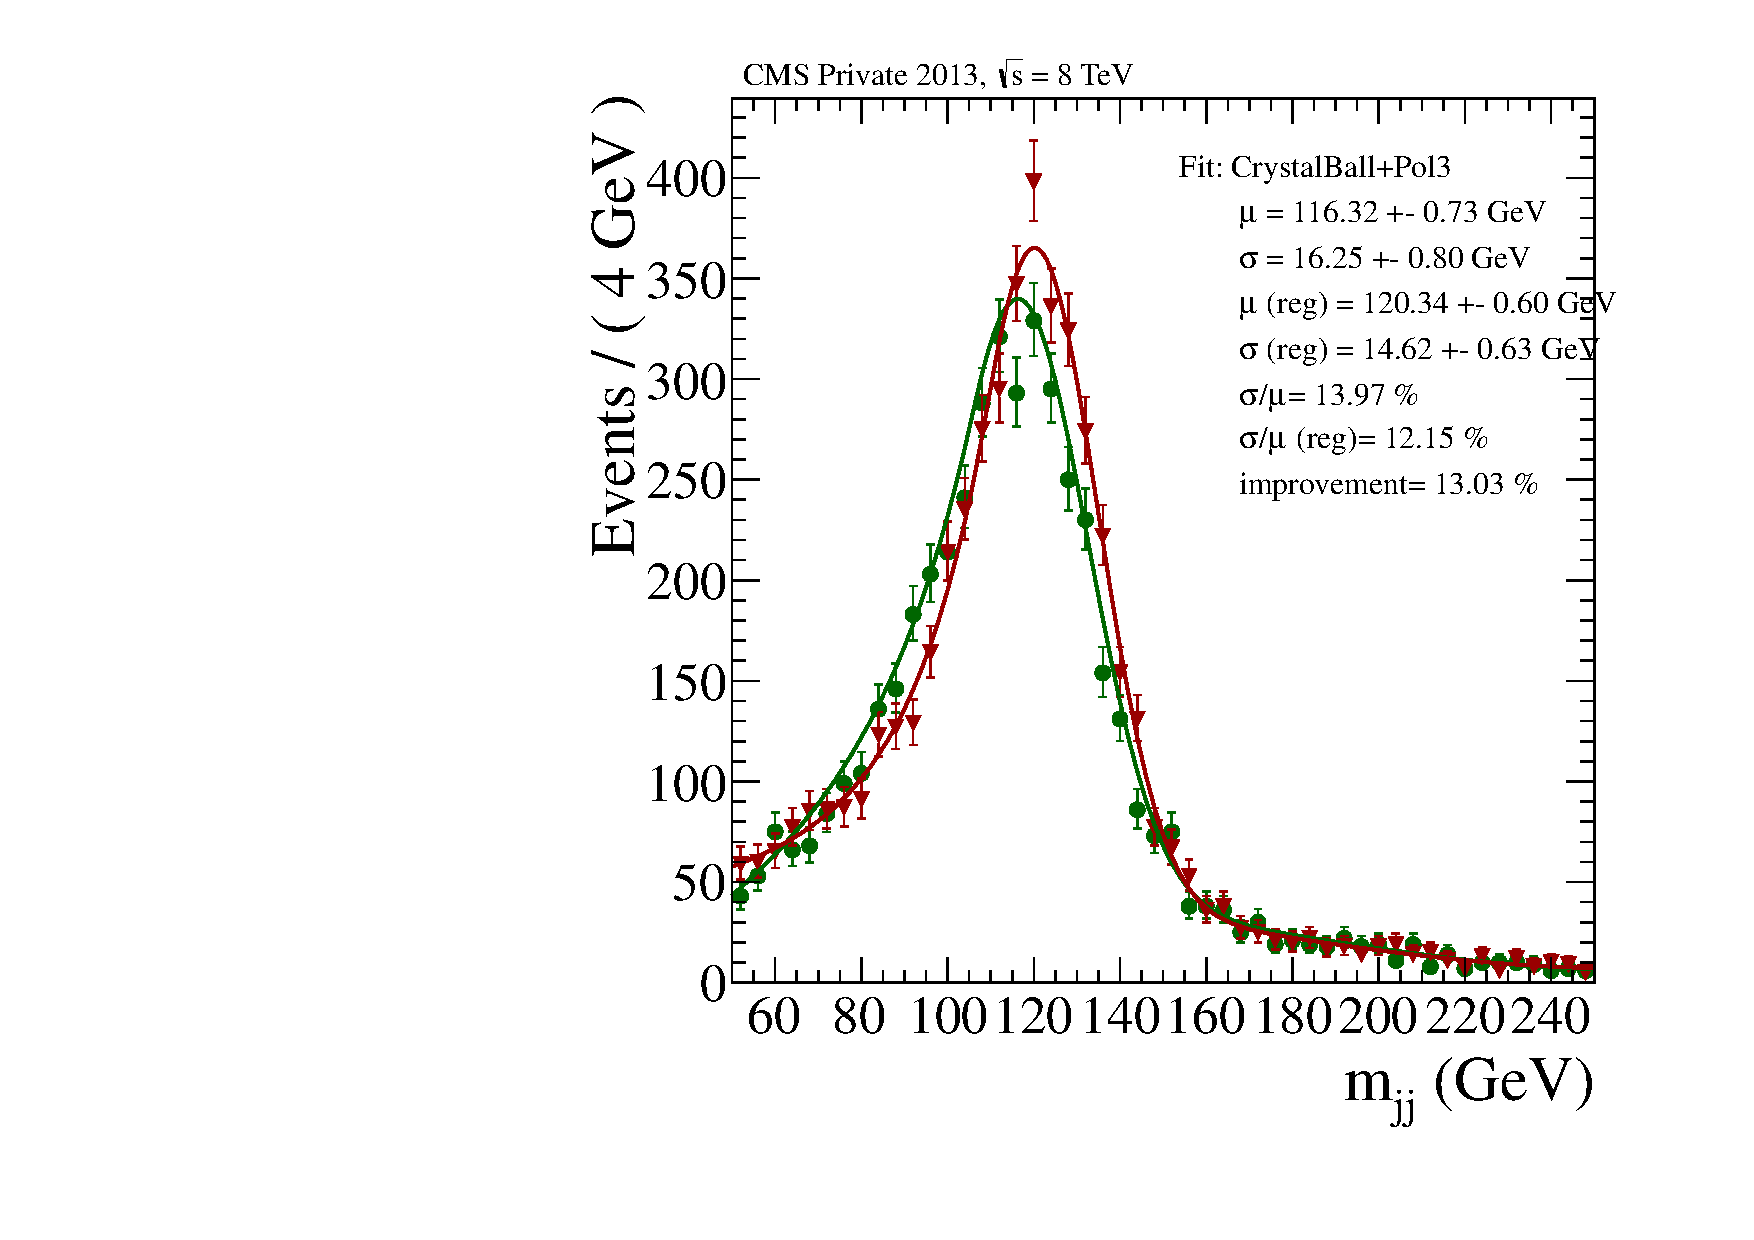
\includegraphics[width=.4\textwidth]{figures/objects/mjj_m270_CrystalBall_allcat.pdf}
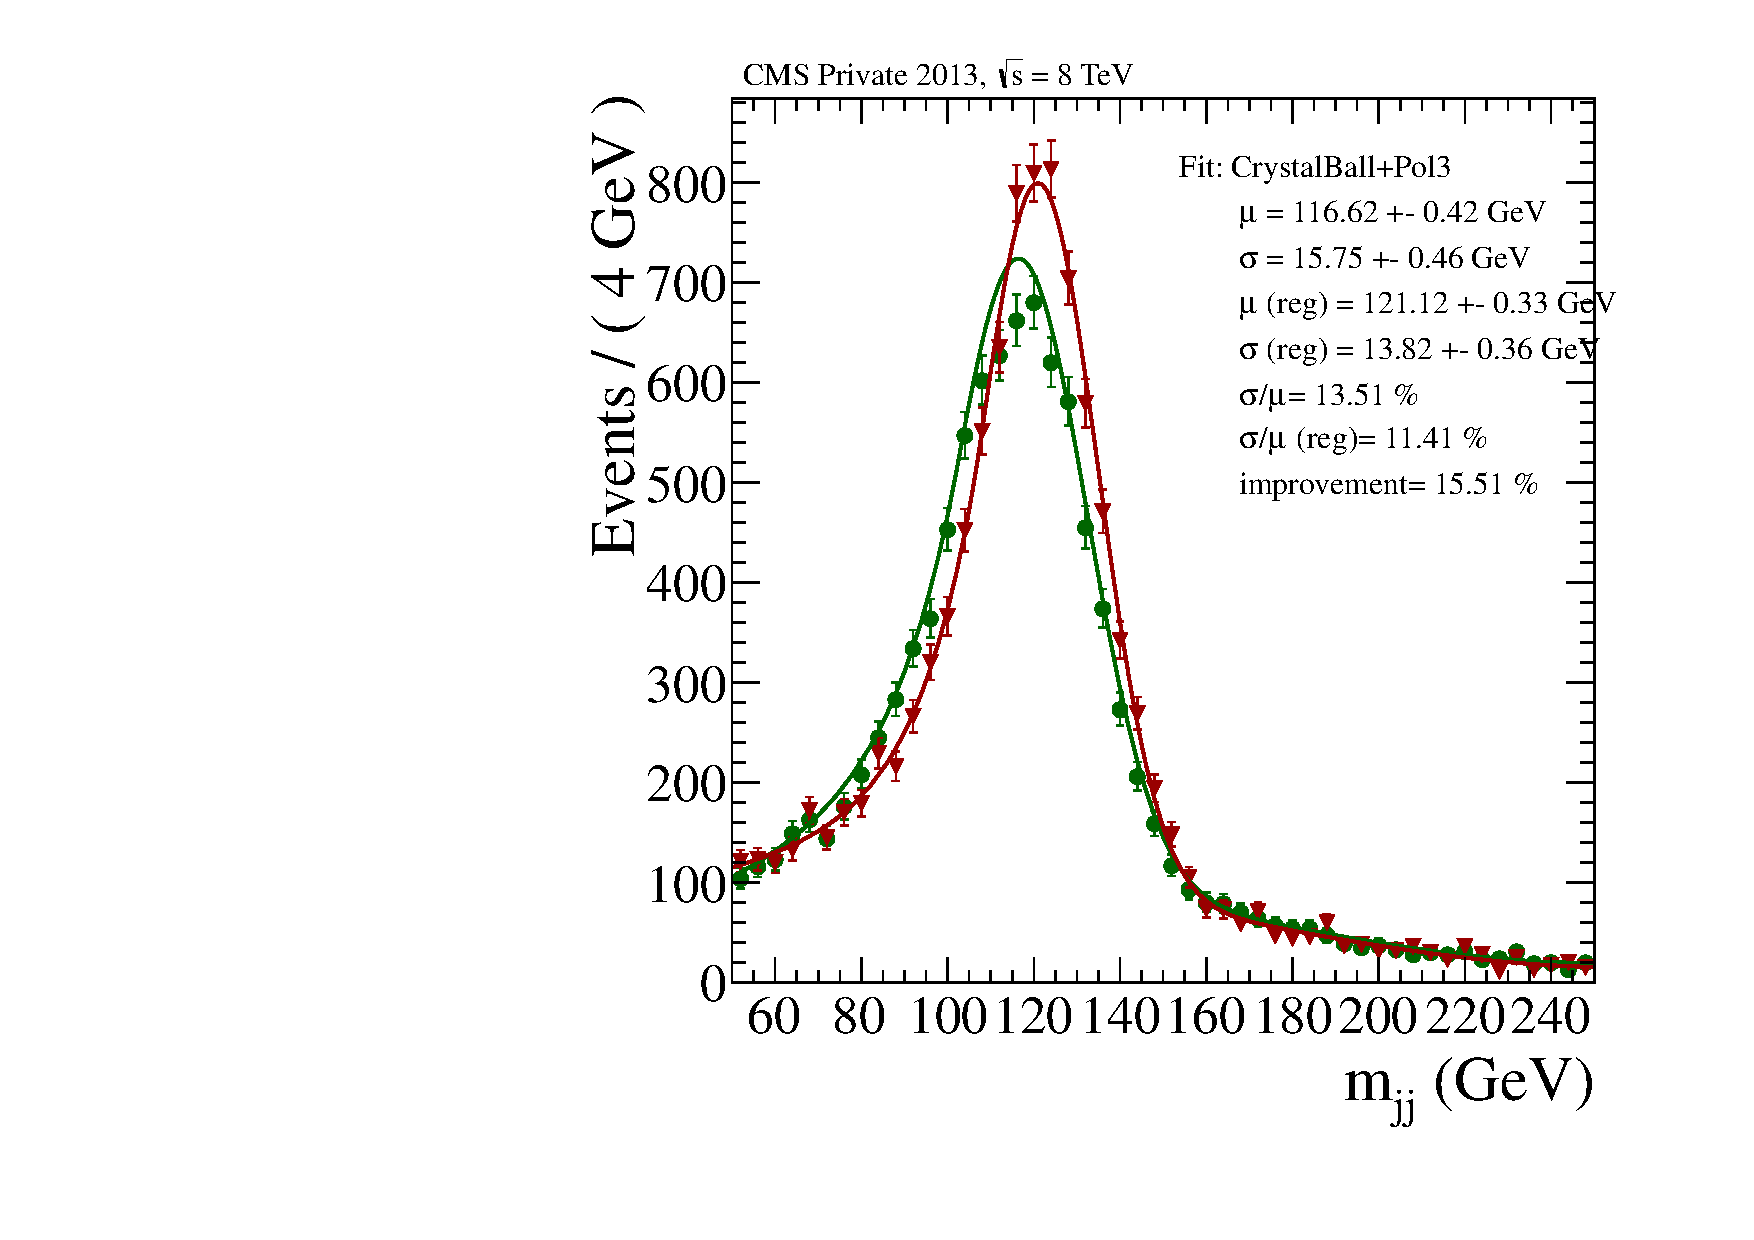
\includegraphics[width=.4\textwidth]{figures/objects/mjj_m300_CrystalBall_allcat.pdf}
\\
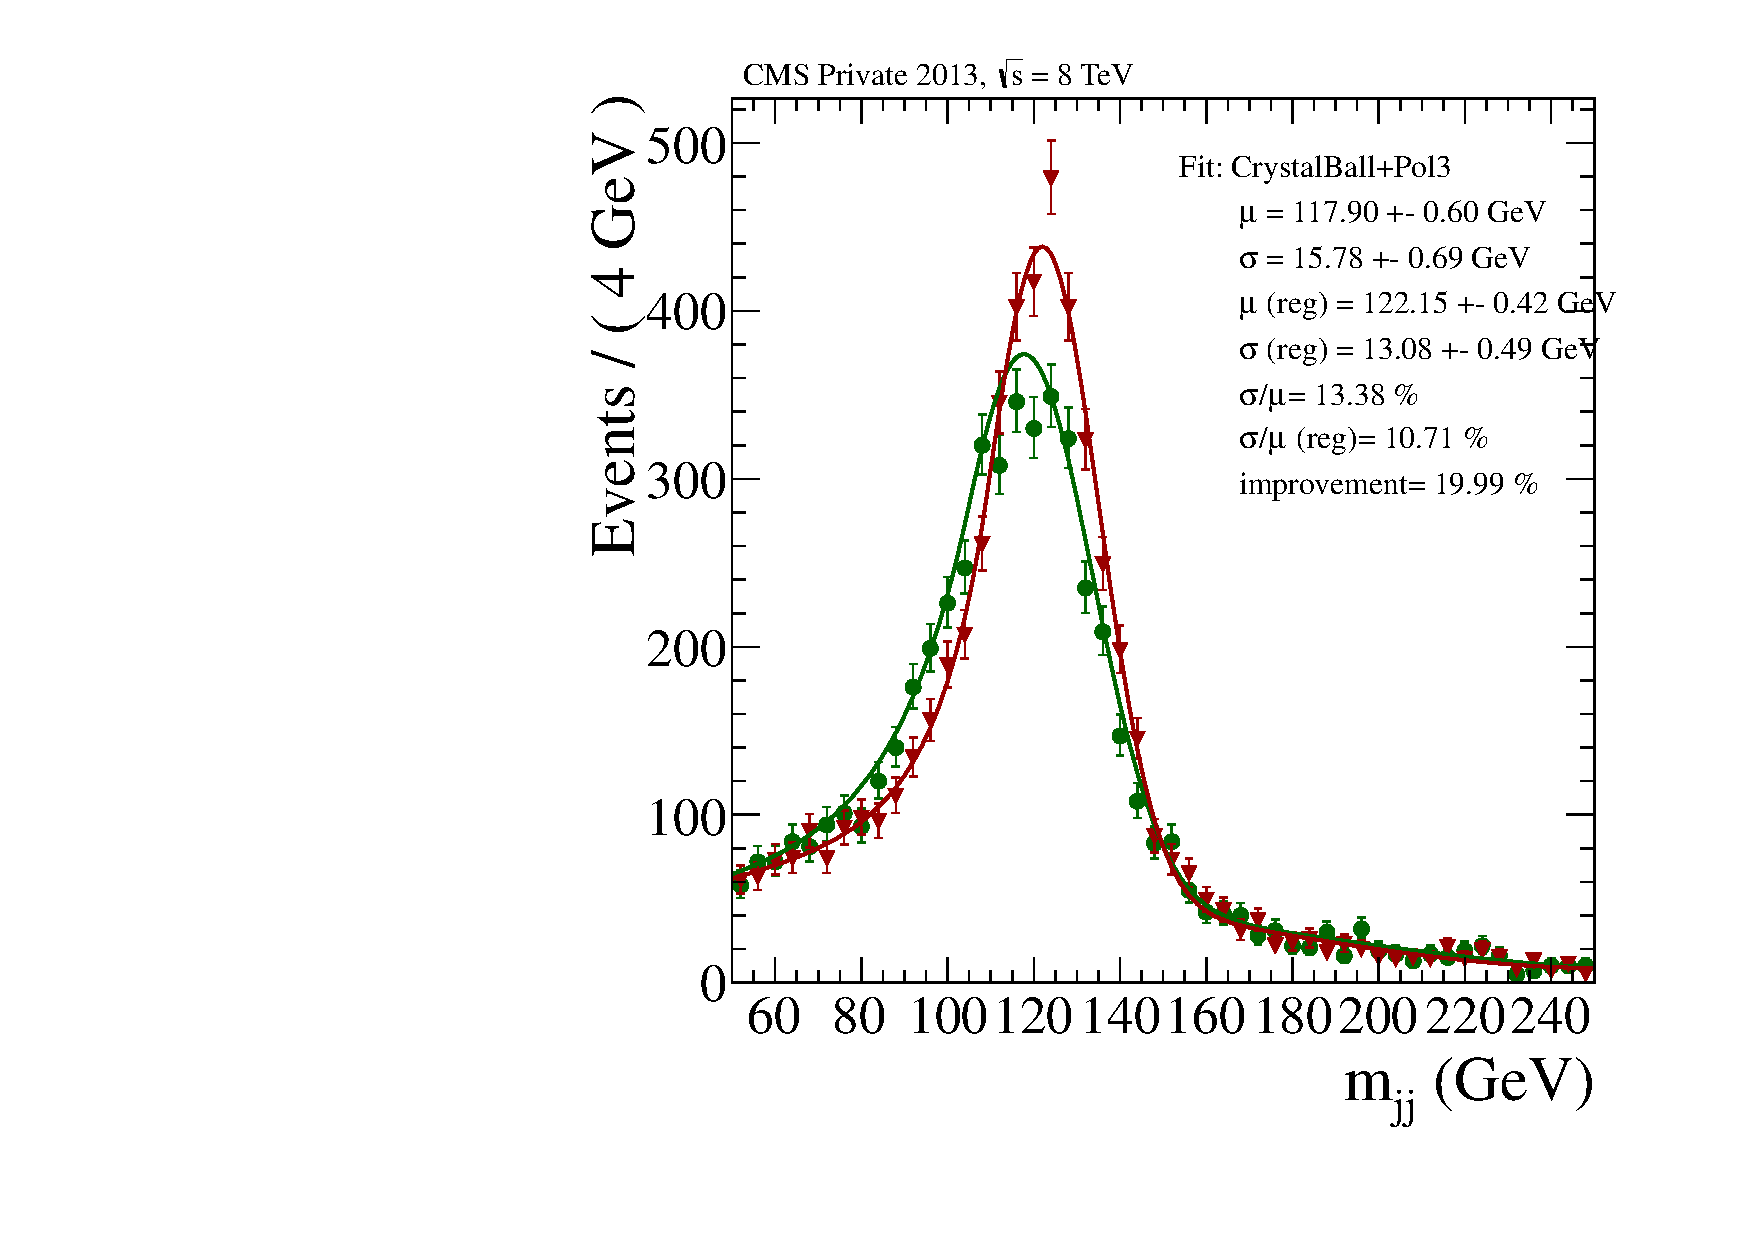
\includegraphics[width=.4\textwidth]{figures/objects/mjj_m350_CrystalBall_allcat.pdf}
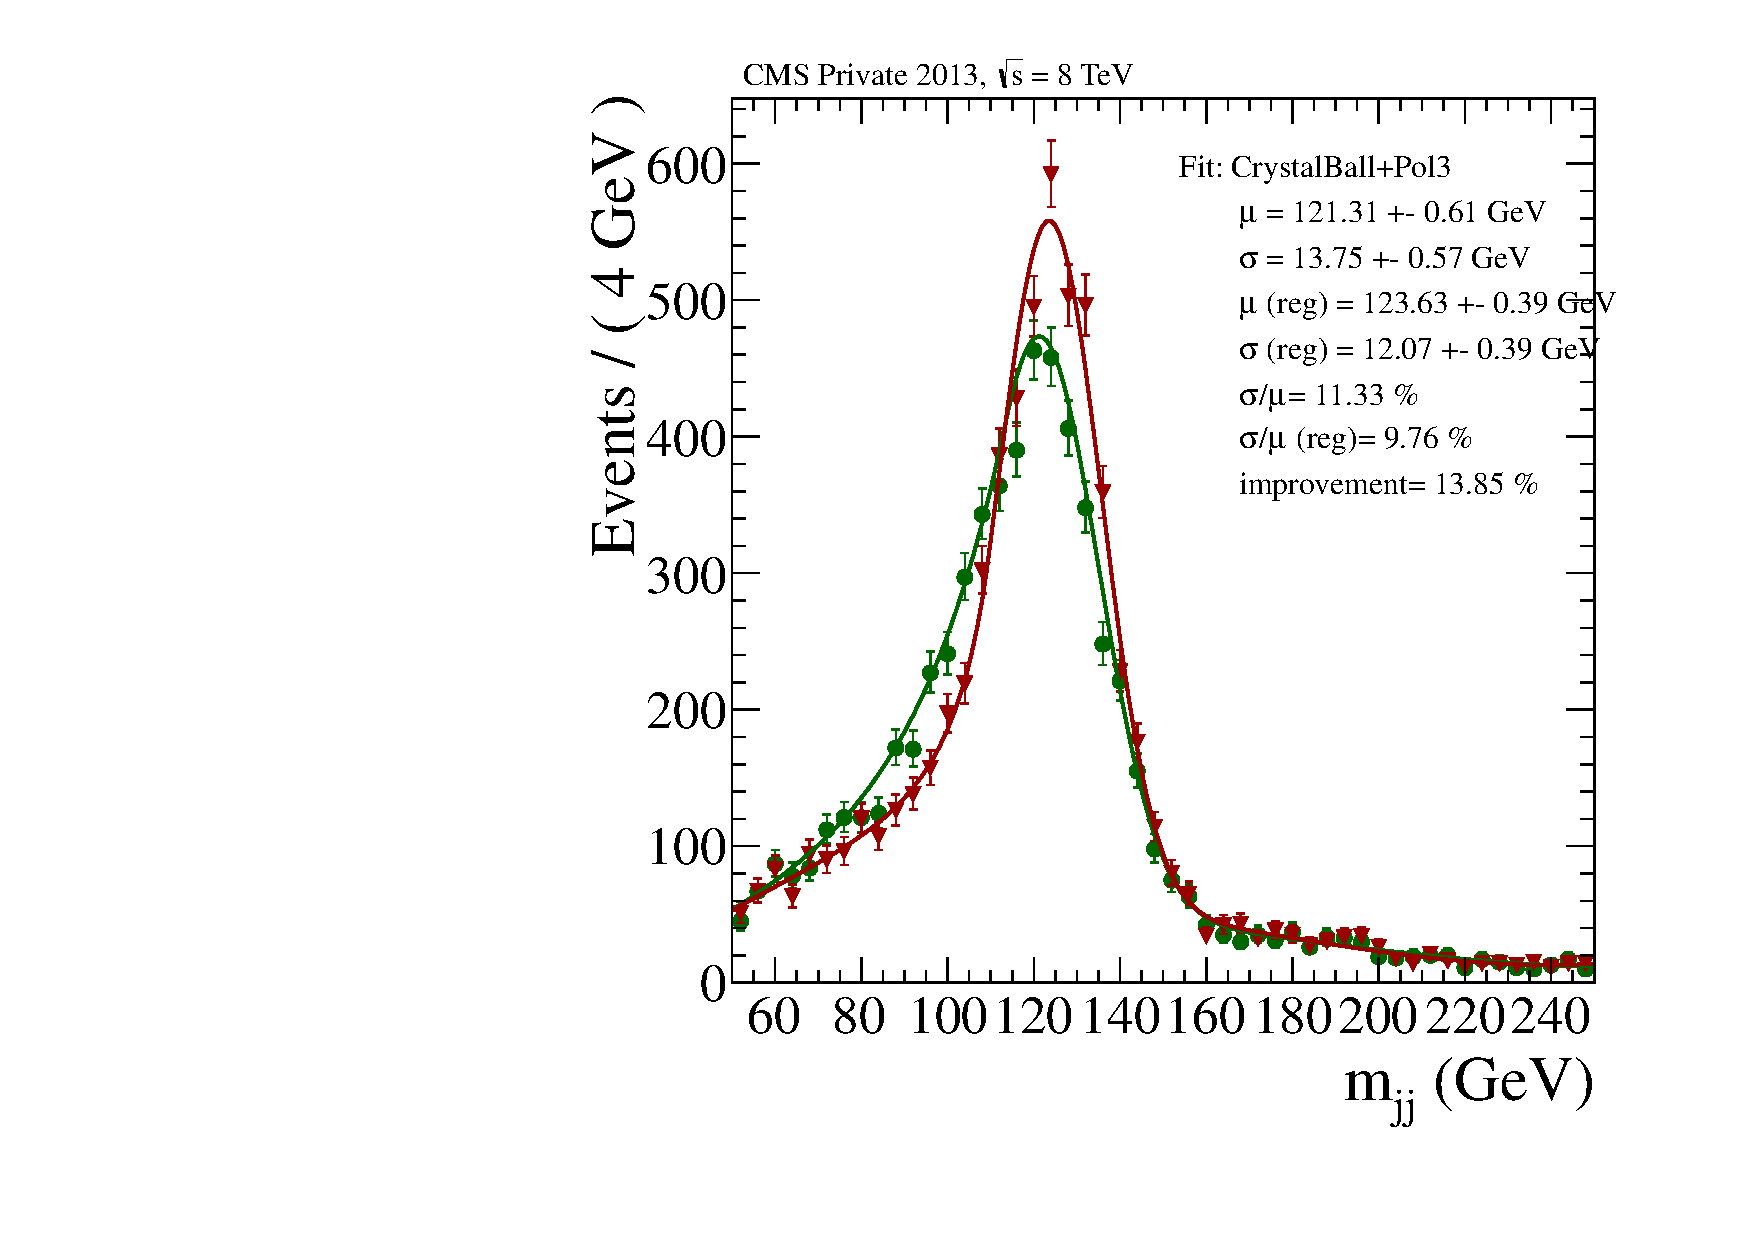
\includegraphics[width=.4\textwidth]{figures/objects/mjj_m400_CrystalBall_allcat.pdf}
\end{center}
\caption{Resolution improvements for the \Mjj\, spectrum at $m_X = 270, 300, 350, 400$~GeV mass points.
The green distribution is before applying the regression, and the red one is after applying the
regression. The fit model is the sum of a Crystal Ball and third-order polynomial.
}
\label{fig:regression_plots_improvement_mjj}
\end{figure}

For validation of the technique, the effect of the regression is studied on data.
Figure~\ref{fig:regression_plots_dataCS_mjj} shows the effect on the data control sample
(a $\gjjj$ sample reweighted to the $\ggjj$ data, discussed in Section~\ref{subsec:dataCS}). The peak
is slightly shifted, and in the region about the Higgs mass, the yield increases about 10\% without
any local peaking structure. 
In addition, comparison between data and the sum of MC backgrounds was performed for the $p_{\rm T}$
balance between the dijet and diphoton candidates before and after regression.
As shown in Figure~\ref{fig:regression_validation_datavsmc}, the ratio
$\frac{p_{{\rm T},jj}}{p_{{\rm T},\gamma\gamma}}$ has peak a more narrow and shifted closer
to 1 after the regression is applied. Although the effect indicates the regression is doing its job,
the data and background processes exhibit a slight overcorrection.

\begin{figure}[ht]
\begin{center}
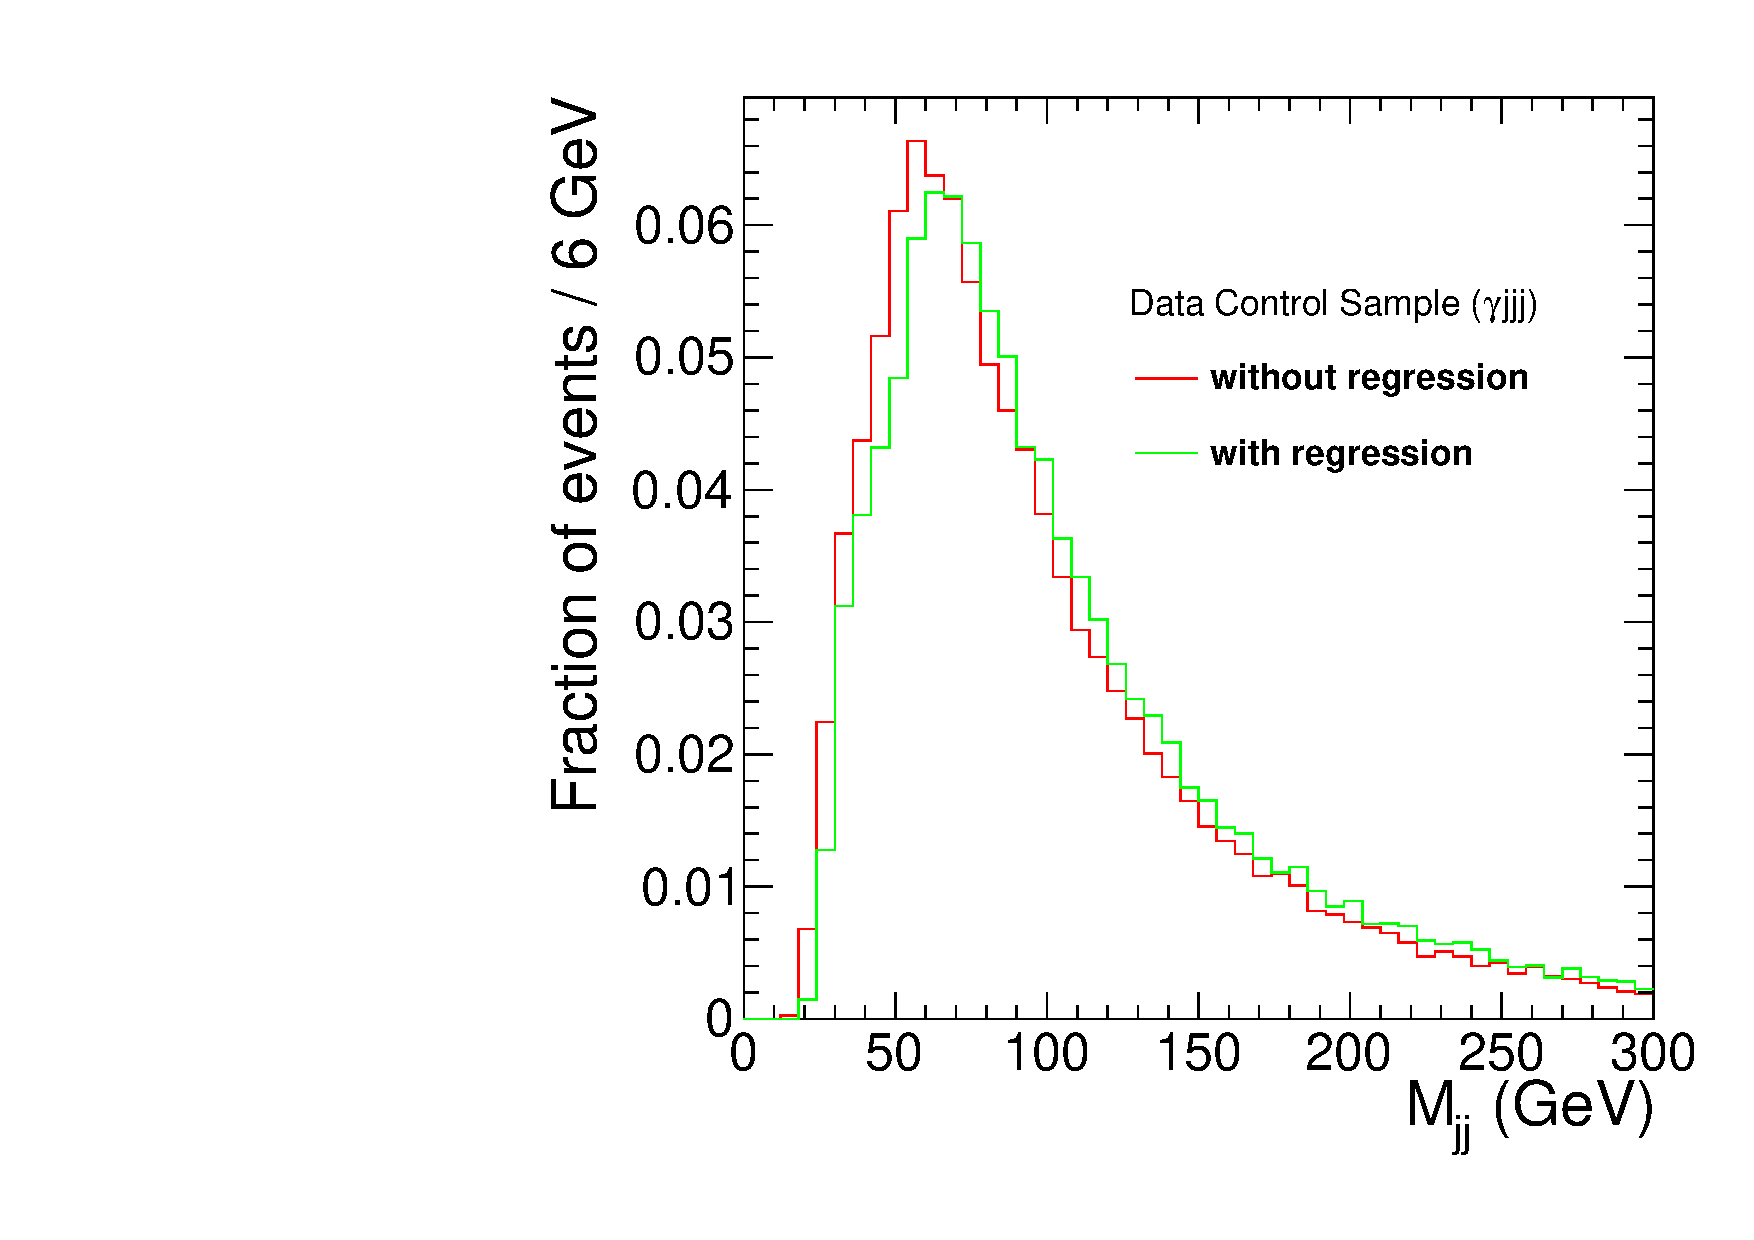
\includegraphics[width=.4\textwidth]{figures/objects/dataCS_mjj.pdf}
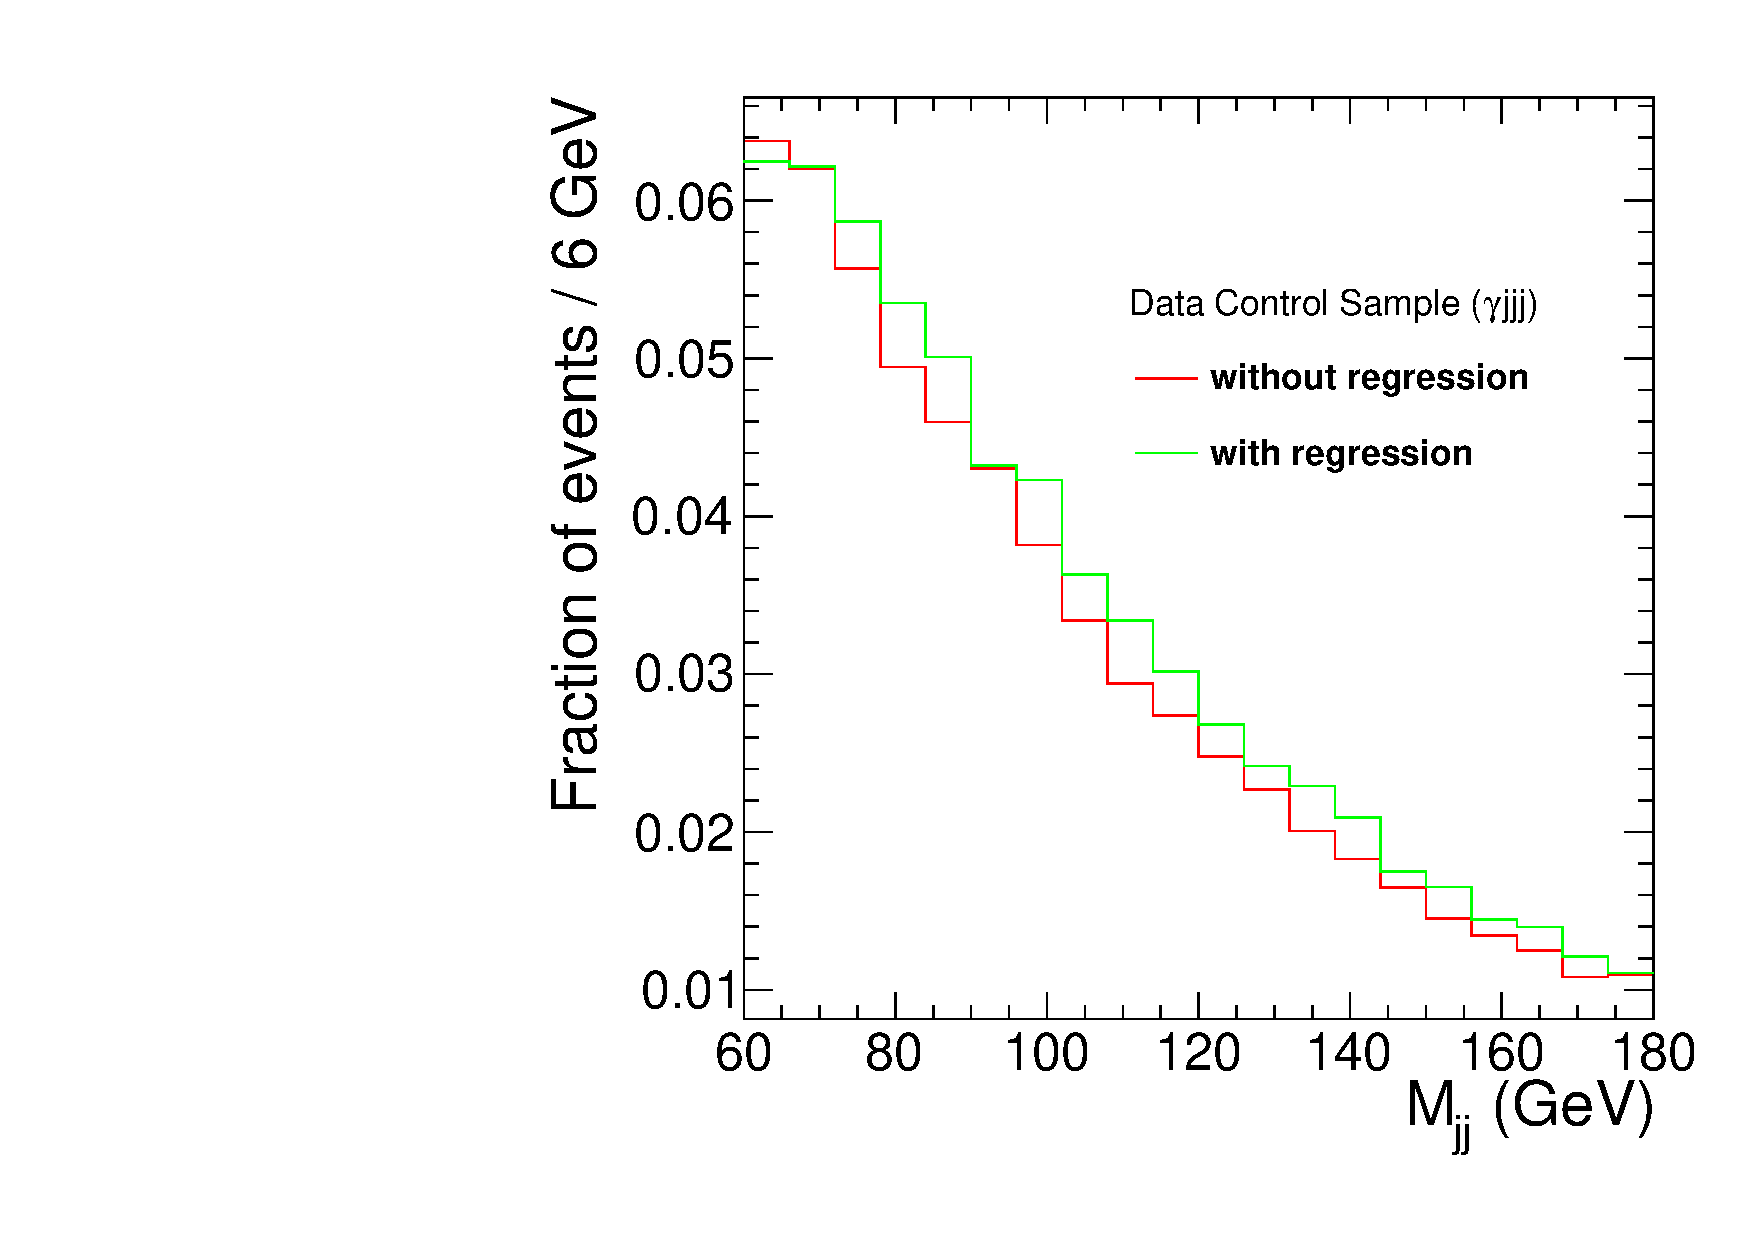
\includegraphics[width=.4\textwidth]{figures/objects/dataCS_mjj_zoom.pdf}
\end{center}
\caption{Effect of regression on the entire \Mjj\, spectrum (left) and zoomed (right)
to a range about the SM Higgs mass on the data control sample, discussed in
Section~\ref{subsec:dataCS}.}
\label{fig:regression_plots_dataCS_mjj} 
\end{figure}

\begin{figure}[ht]
\begin{center}
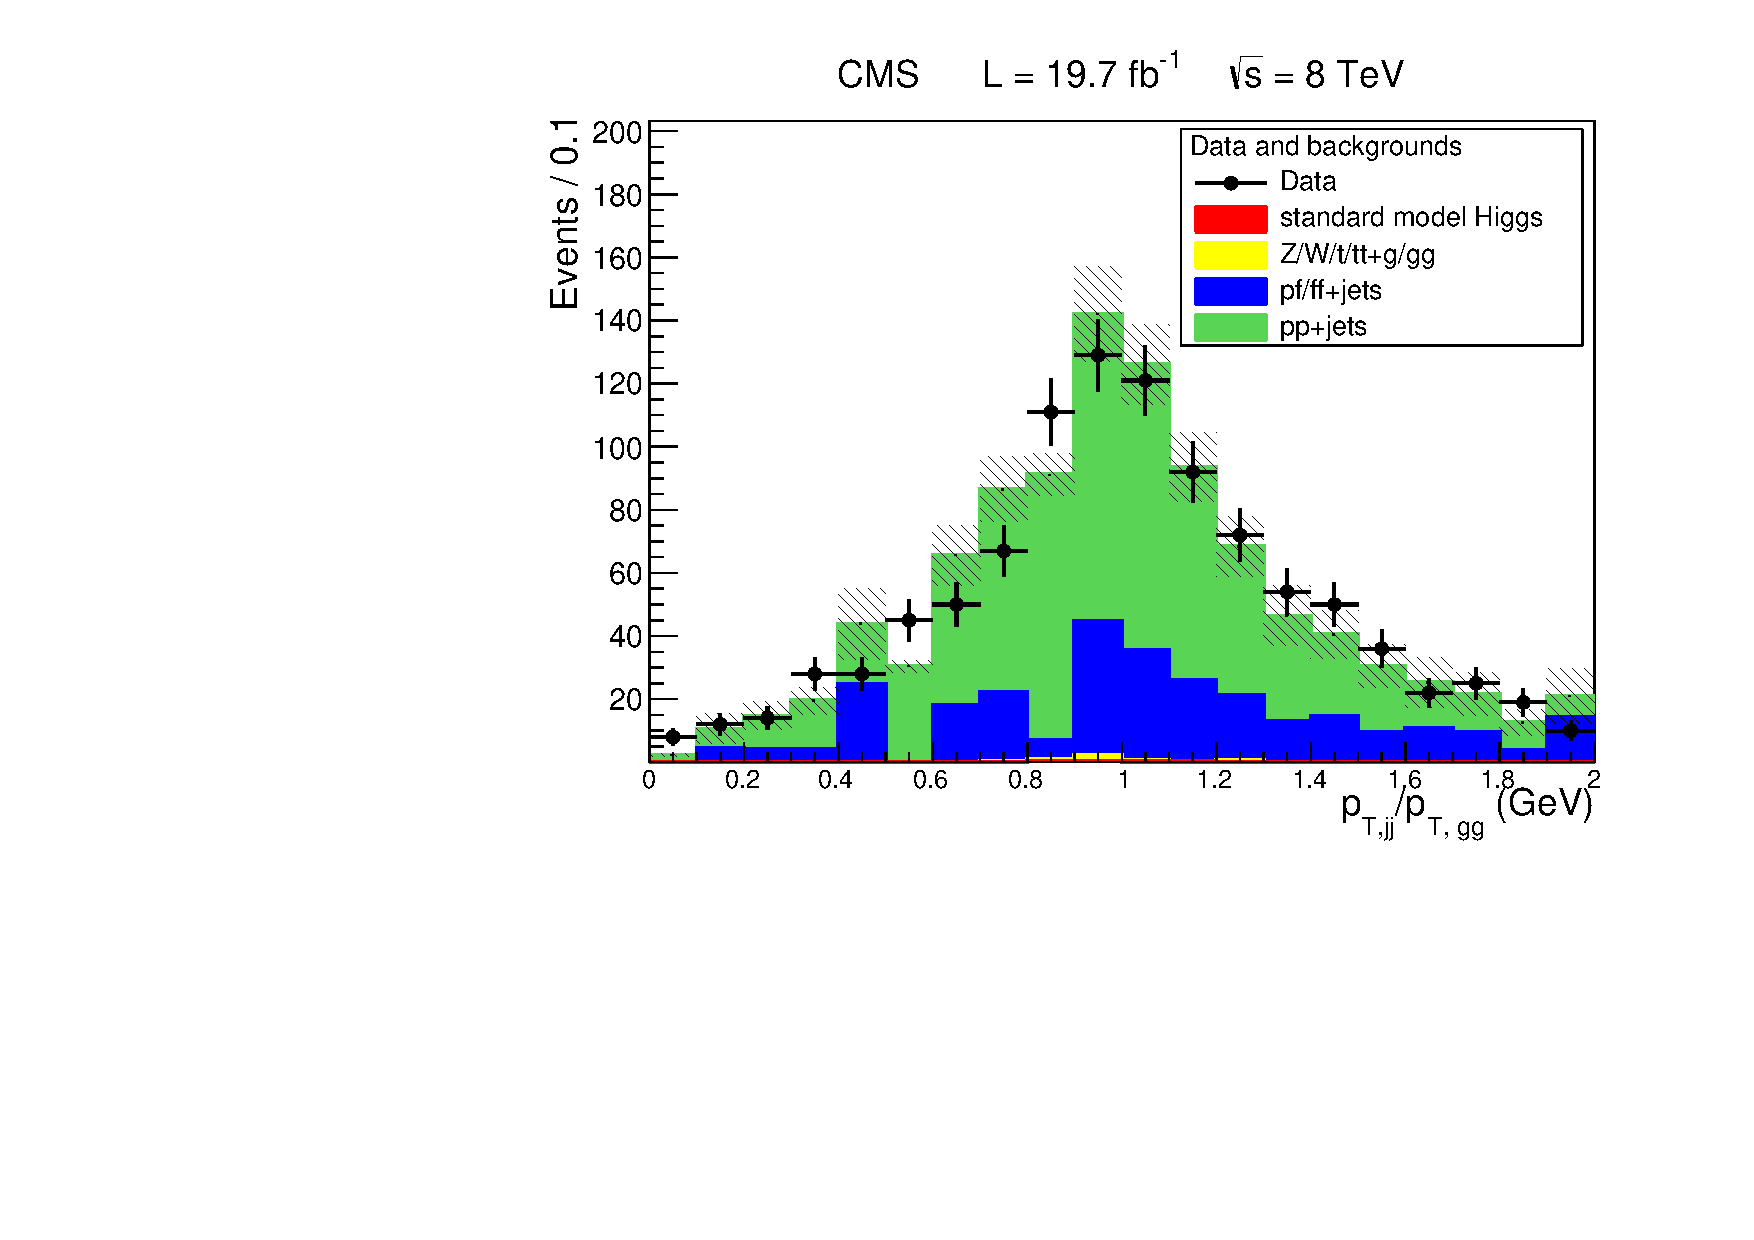
\includegraphics[width=.7\textwidth]{figures/objects/pt_balance_datavsmc_before.pdf}
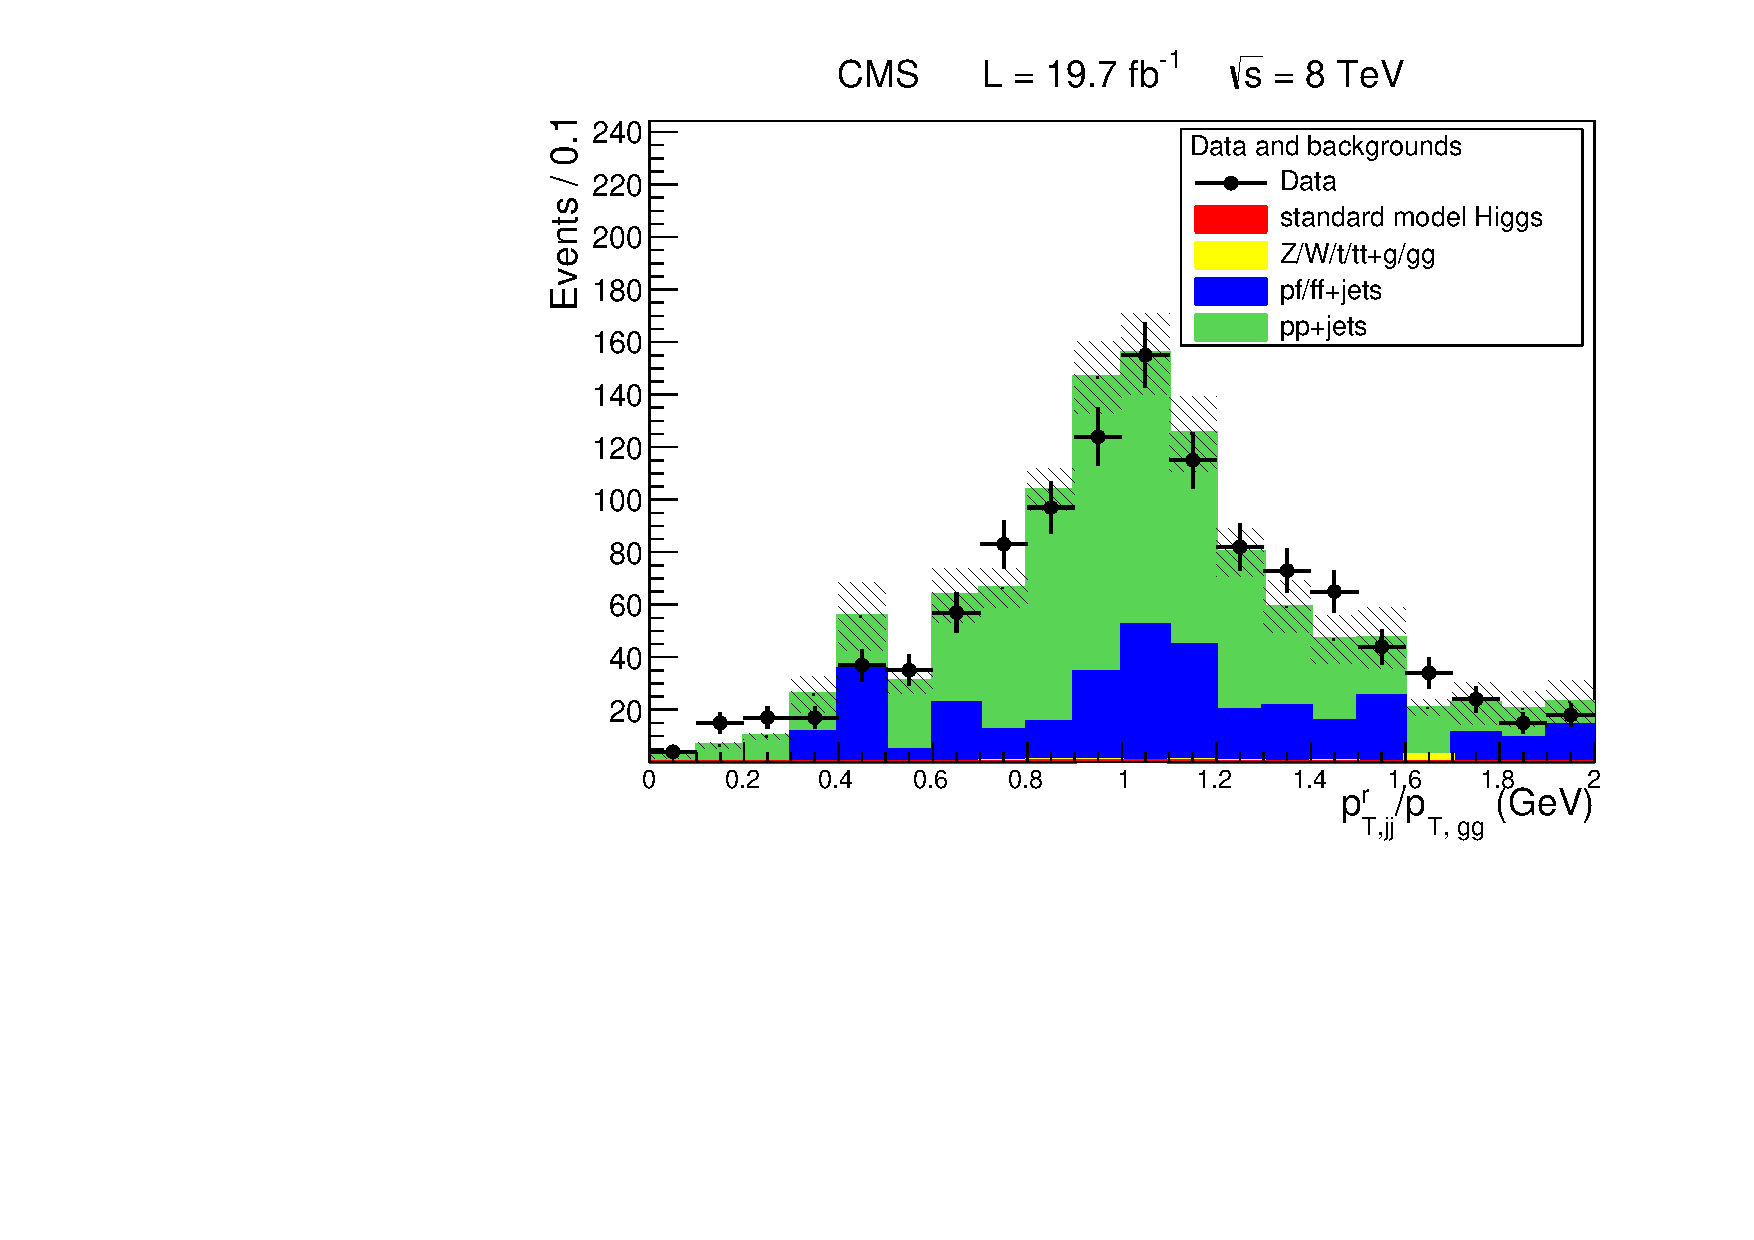
\includegraphics[width=.7\textwidth]{figures/objects/pt_balance_datavsmc_after.pdf}
\end{center}
\caption{Improvement in the $p_{\rm T}$ balance before (top) and after (bottom) the regression is
applied for a comparison between data and the sum of background processes. The events are a combination
of the 1-tag and 2-tag categories with an additional requirement that there be no jets other than
the two from the $\Hbb$ decay.}
\label{fig:regression_validation_datavsmc} 
\end{figure}
